\fhooelecture[Ein IoT-System zur Wasserüberwachung]{\Huge Ein IoT-System zur Wasserüberwachung}{Ein IoT-System zur Wasserüberwachung}{WMIoTS}

\begin{frame}{Erinnerung: Vision für ein Wasser-Monitoring-System}
    \begin{center}
       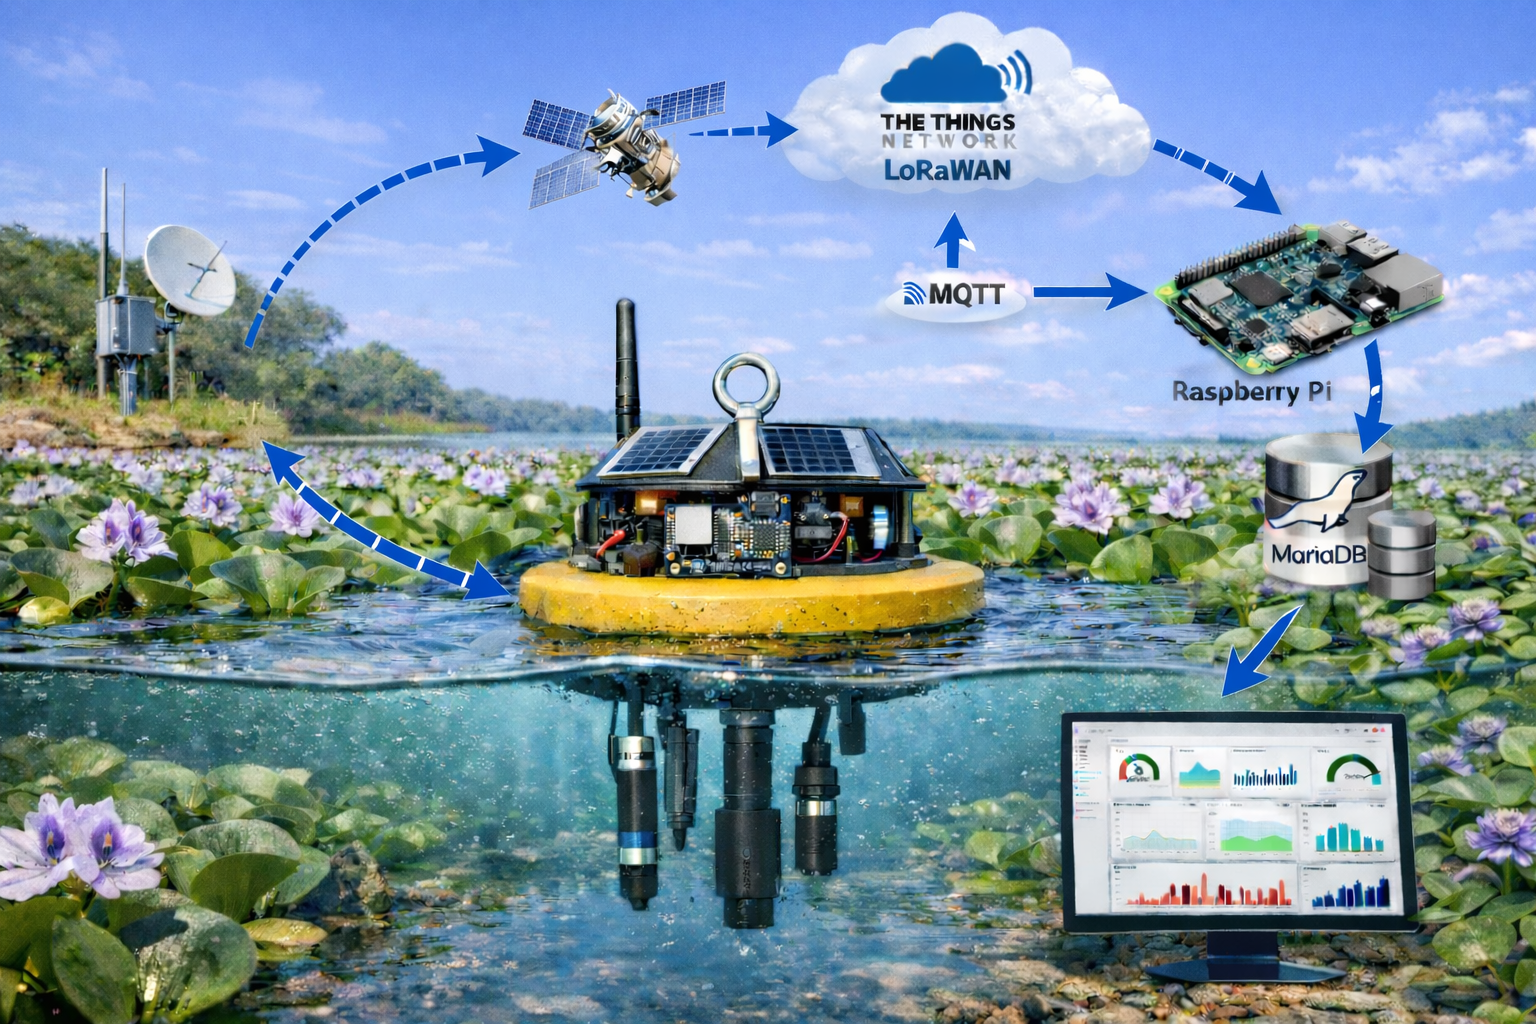
\includegraphics[width=0.74\textwidth]{material/ChatGPT Image Jan 25, 2026, 12_45_31 AM}
    \end{center}
\end{frame}

\part{Work in Progress}

\section[nosectionpage]{Alle Studierende haben der Veröffentlichung der Fotos zugestimmt}

\setbeamercolor{normal text}{bg=black}
\begin{frame}[plain]%
    \makebox[\linewidth]{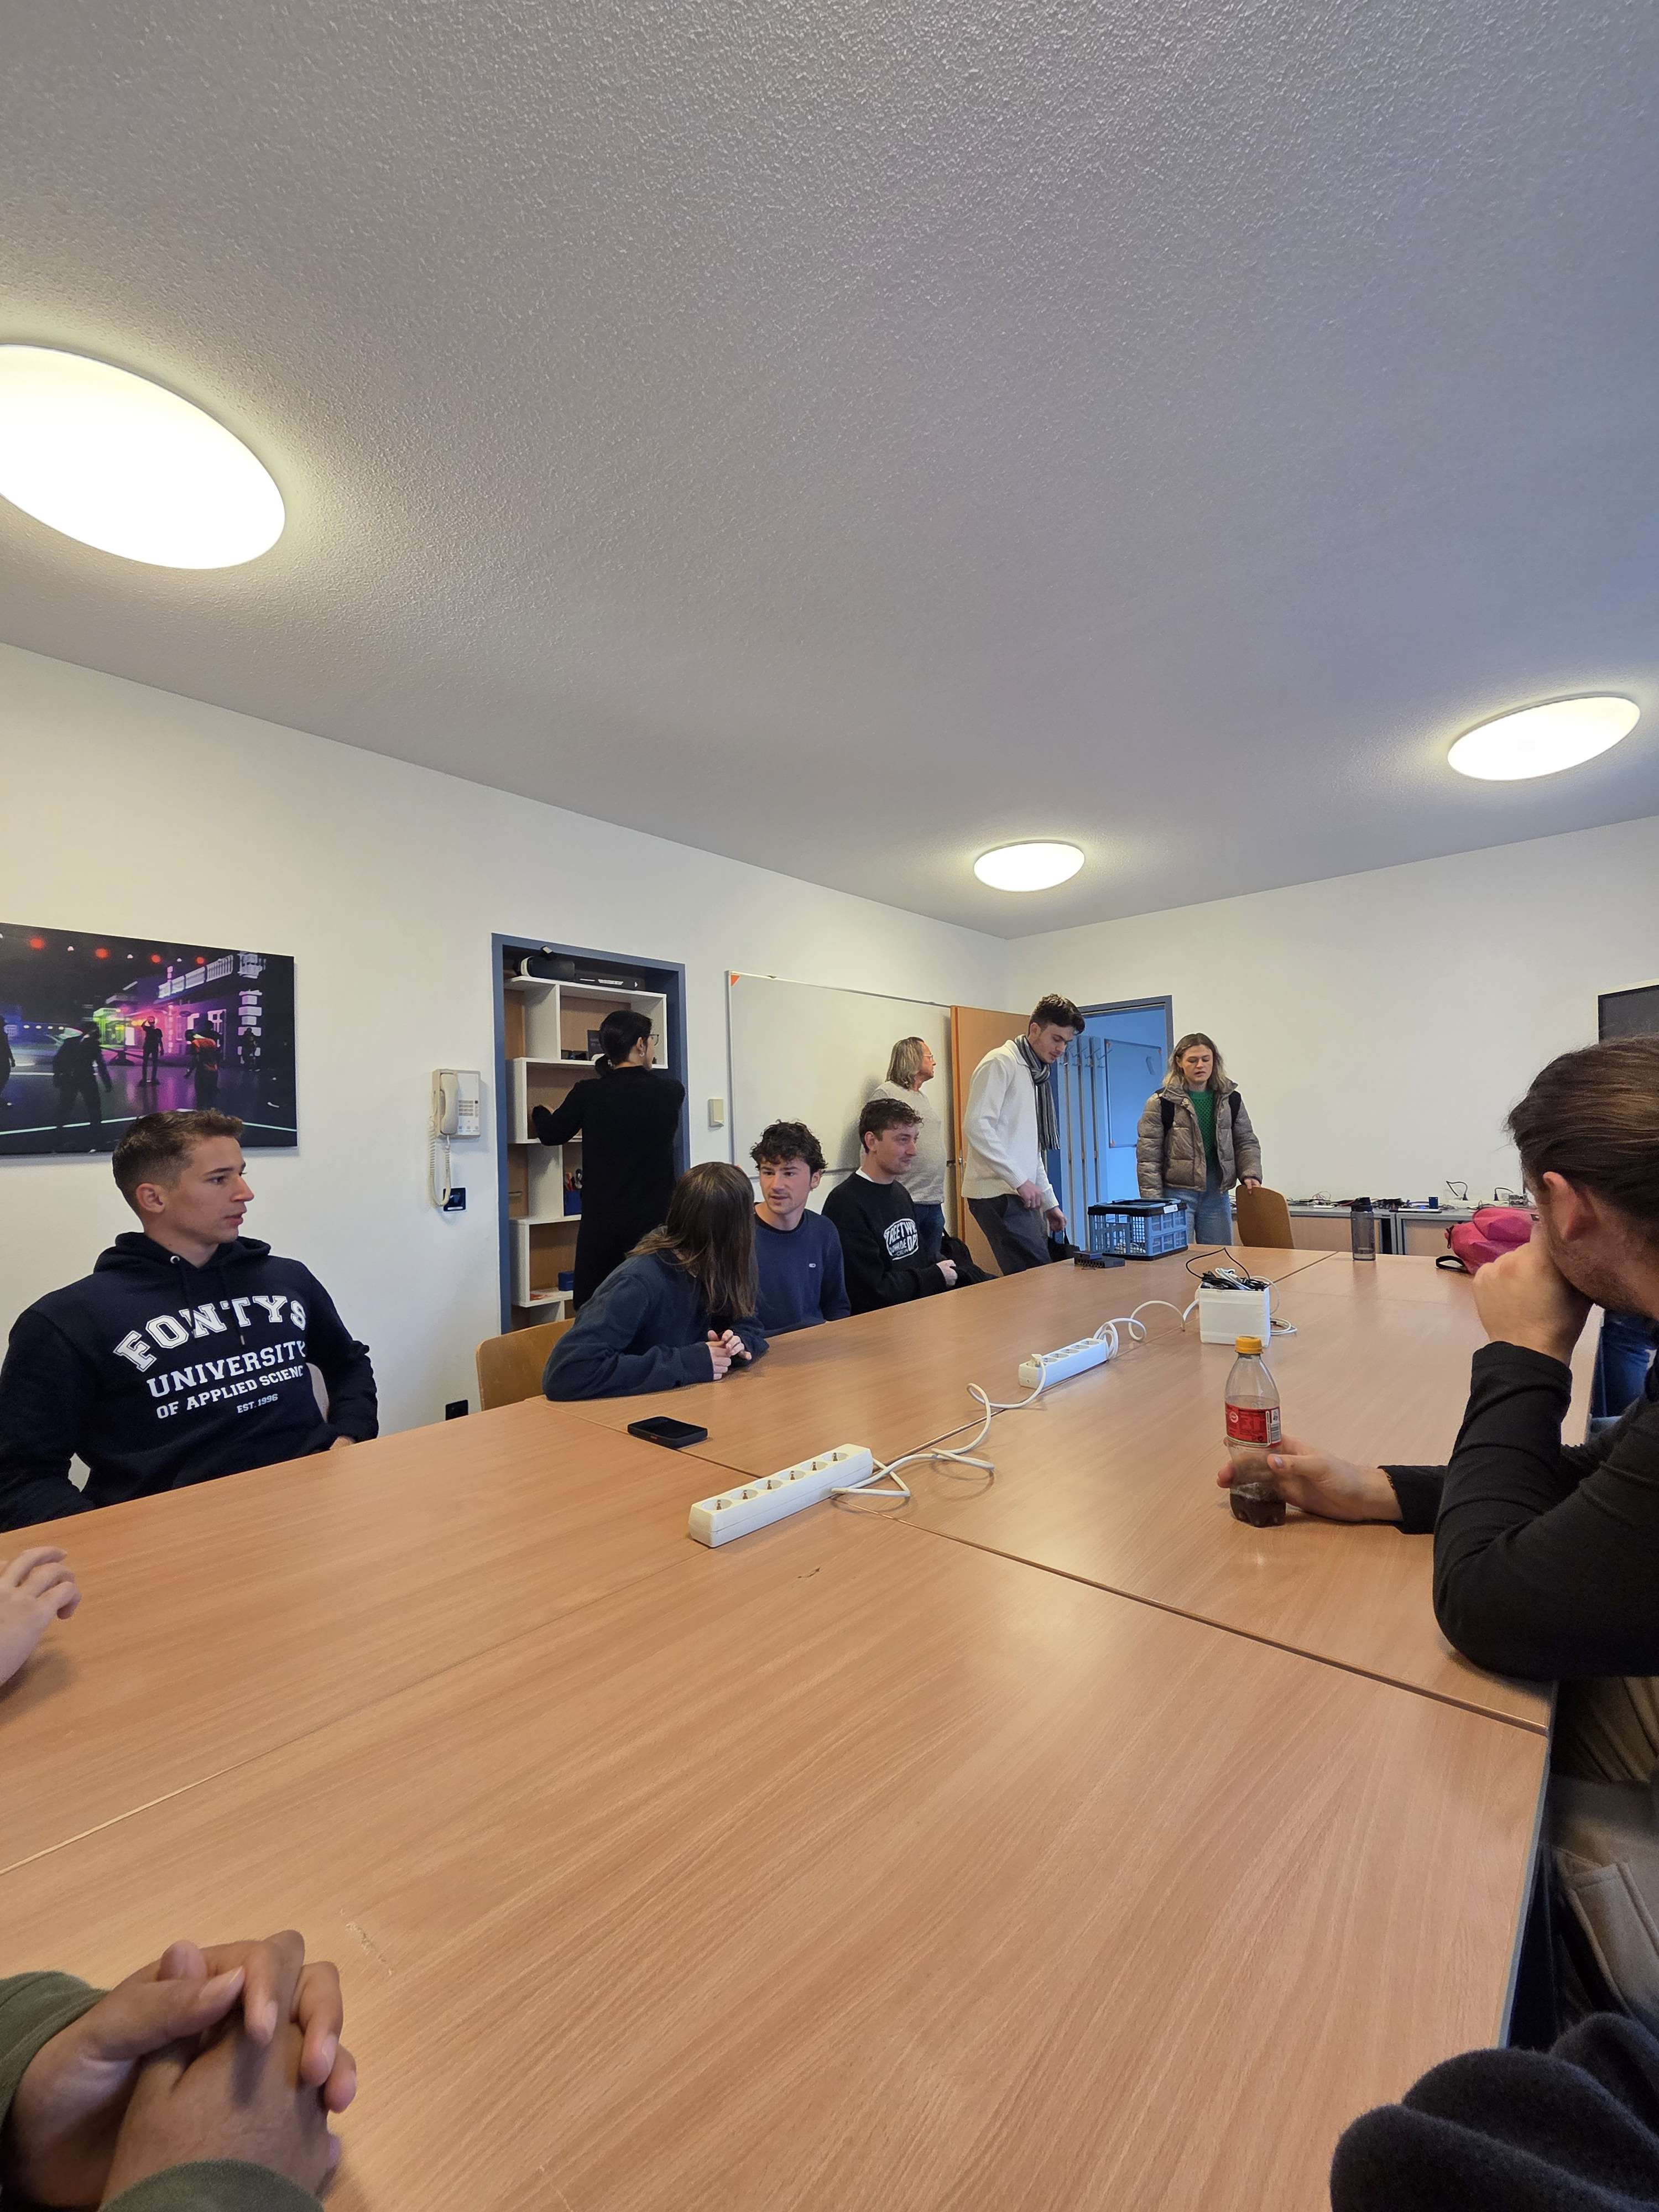
\includegraphics[width=\paperwidth,height=\paperheight,keepaspectratio]{material/A}}%
\end{frame}%
\begin{frame}[plain]
    \makebox[\linewidth]{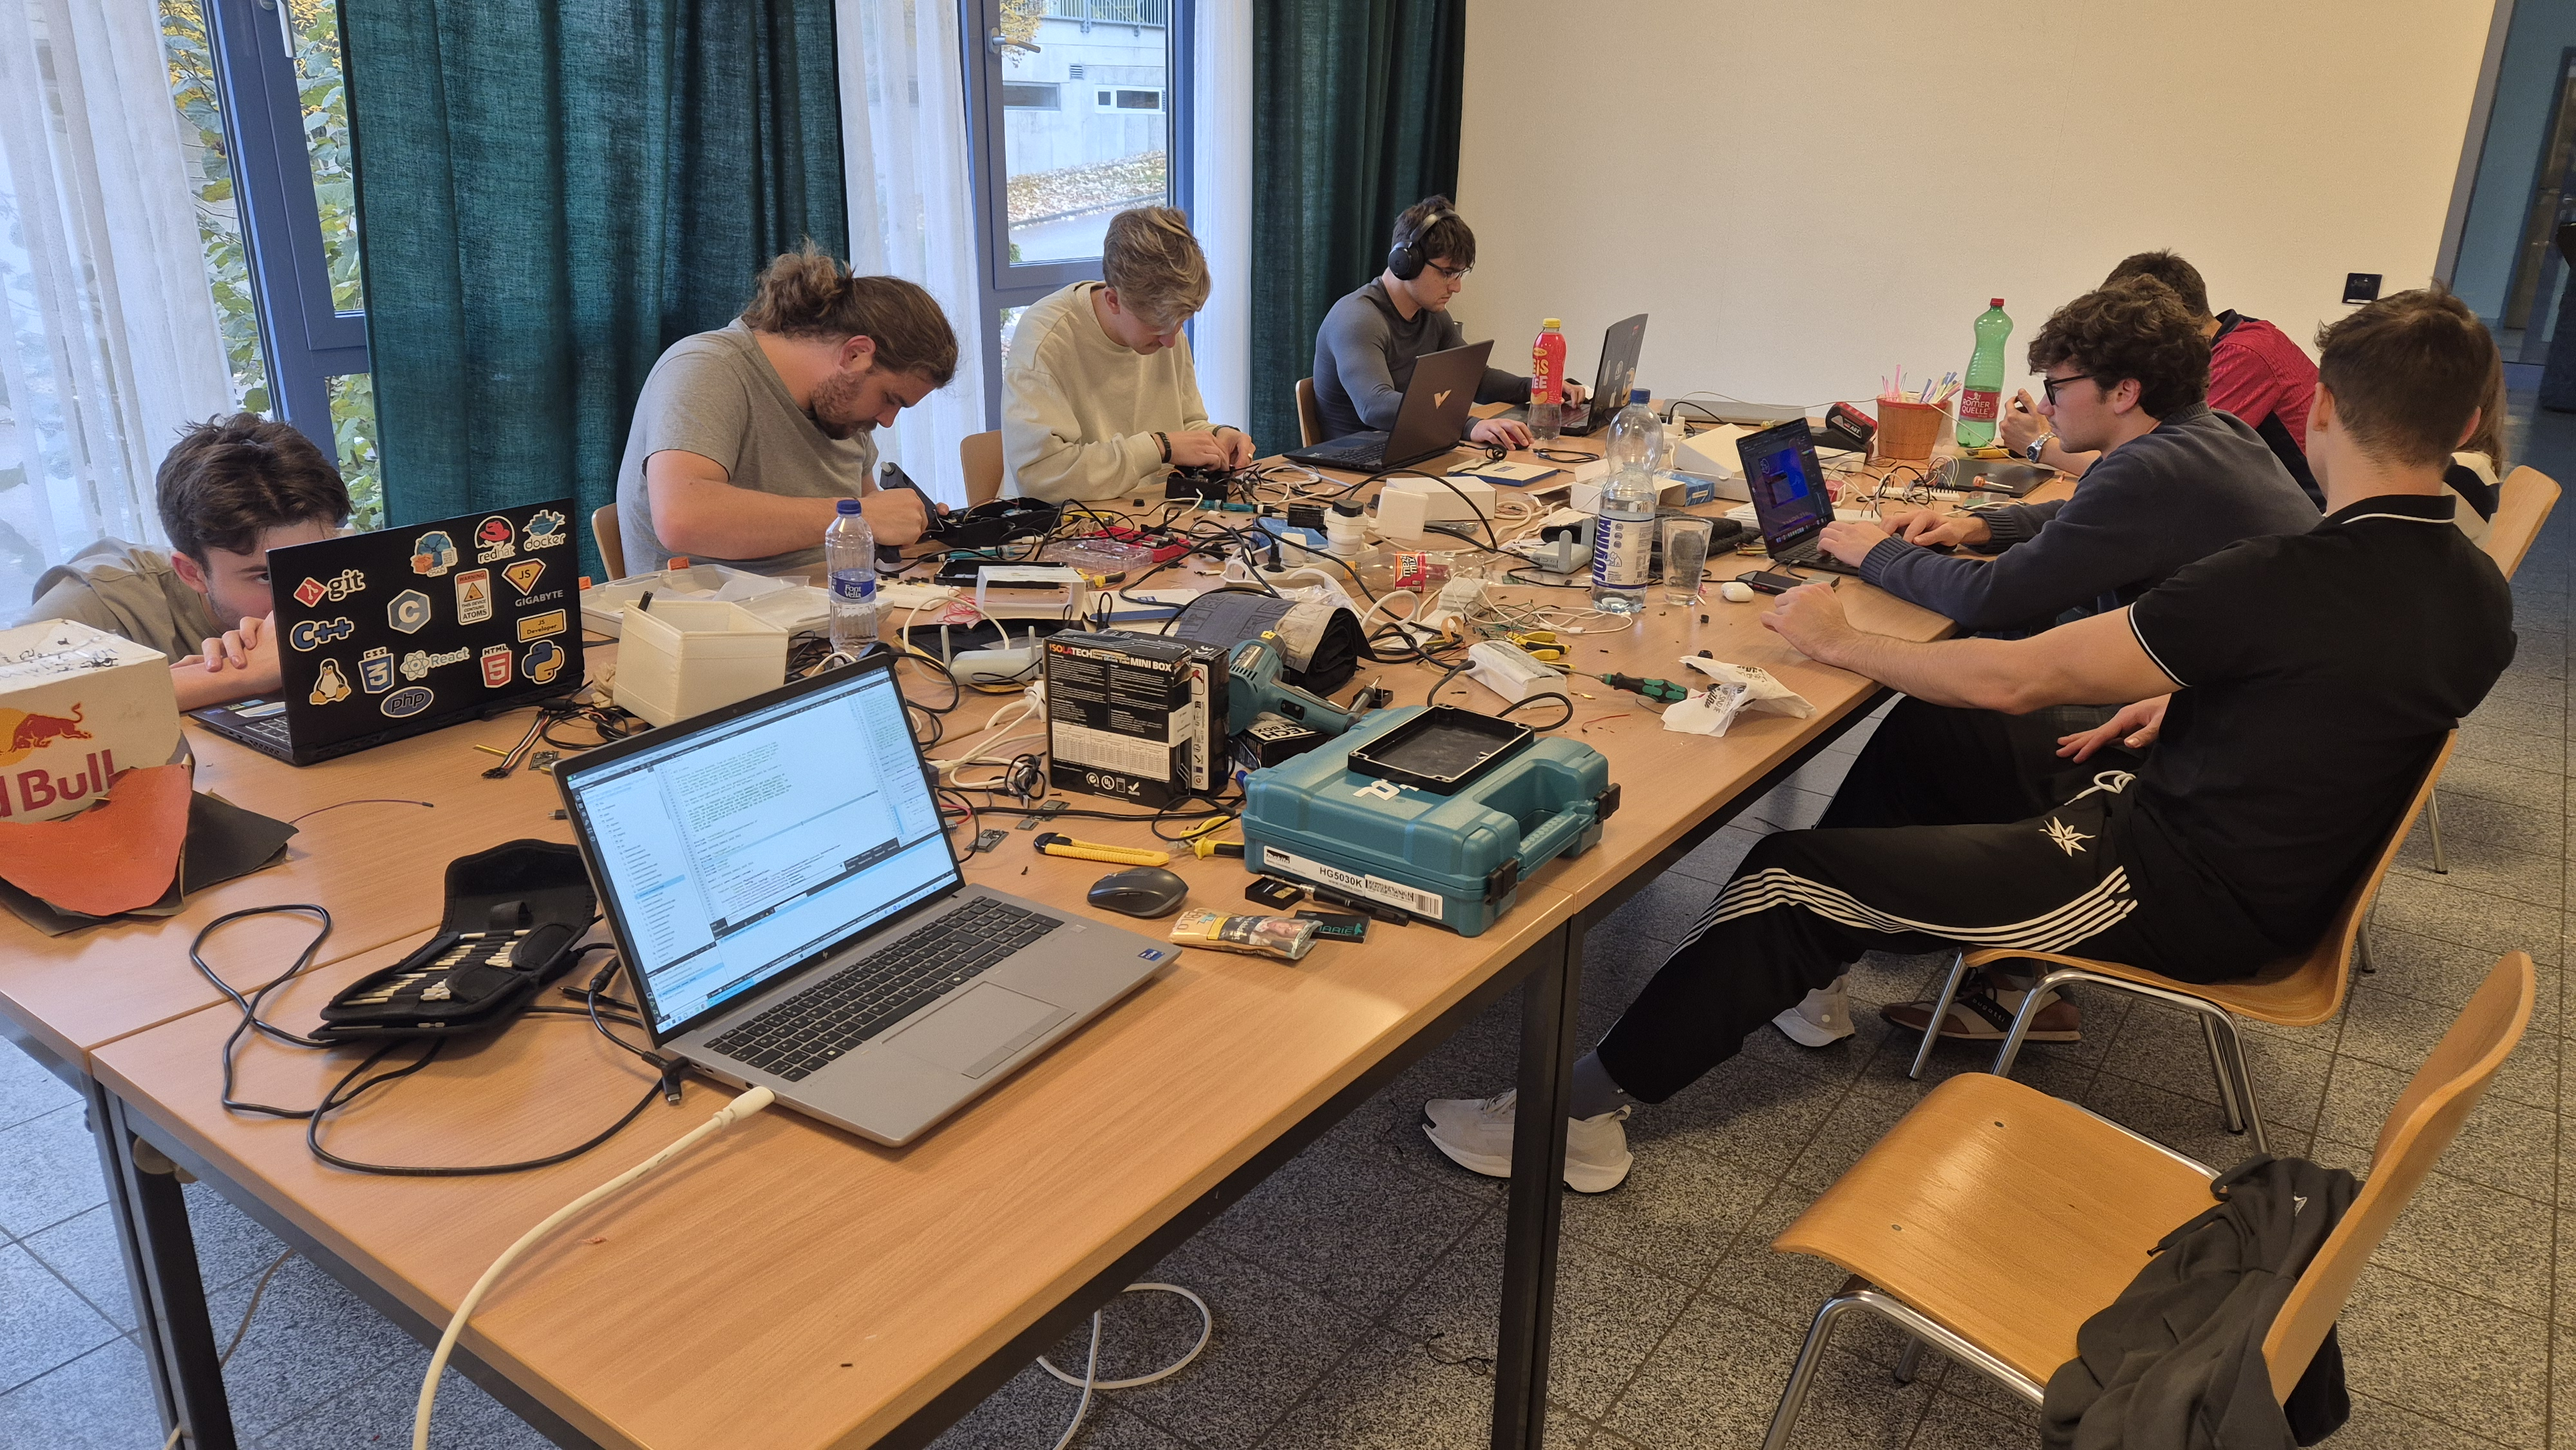
\includegraphics[width=\paperwidth,height=\paperheight,keepaspectratio]{material/B}}%
\end{frame}
\begin{frame}[plain]
    \makebox[\linewidth]{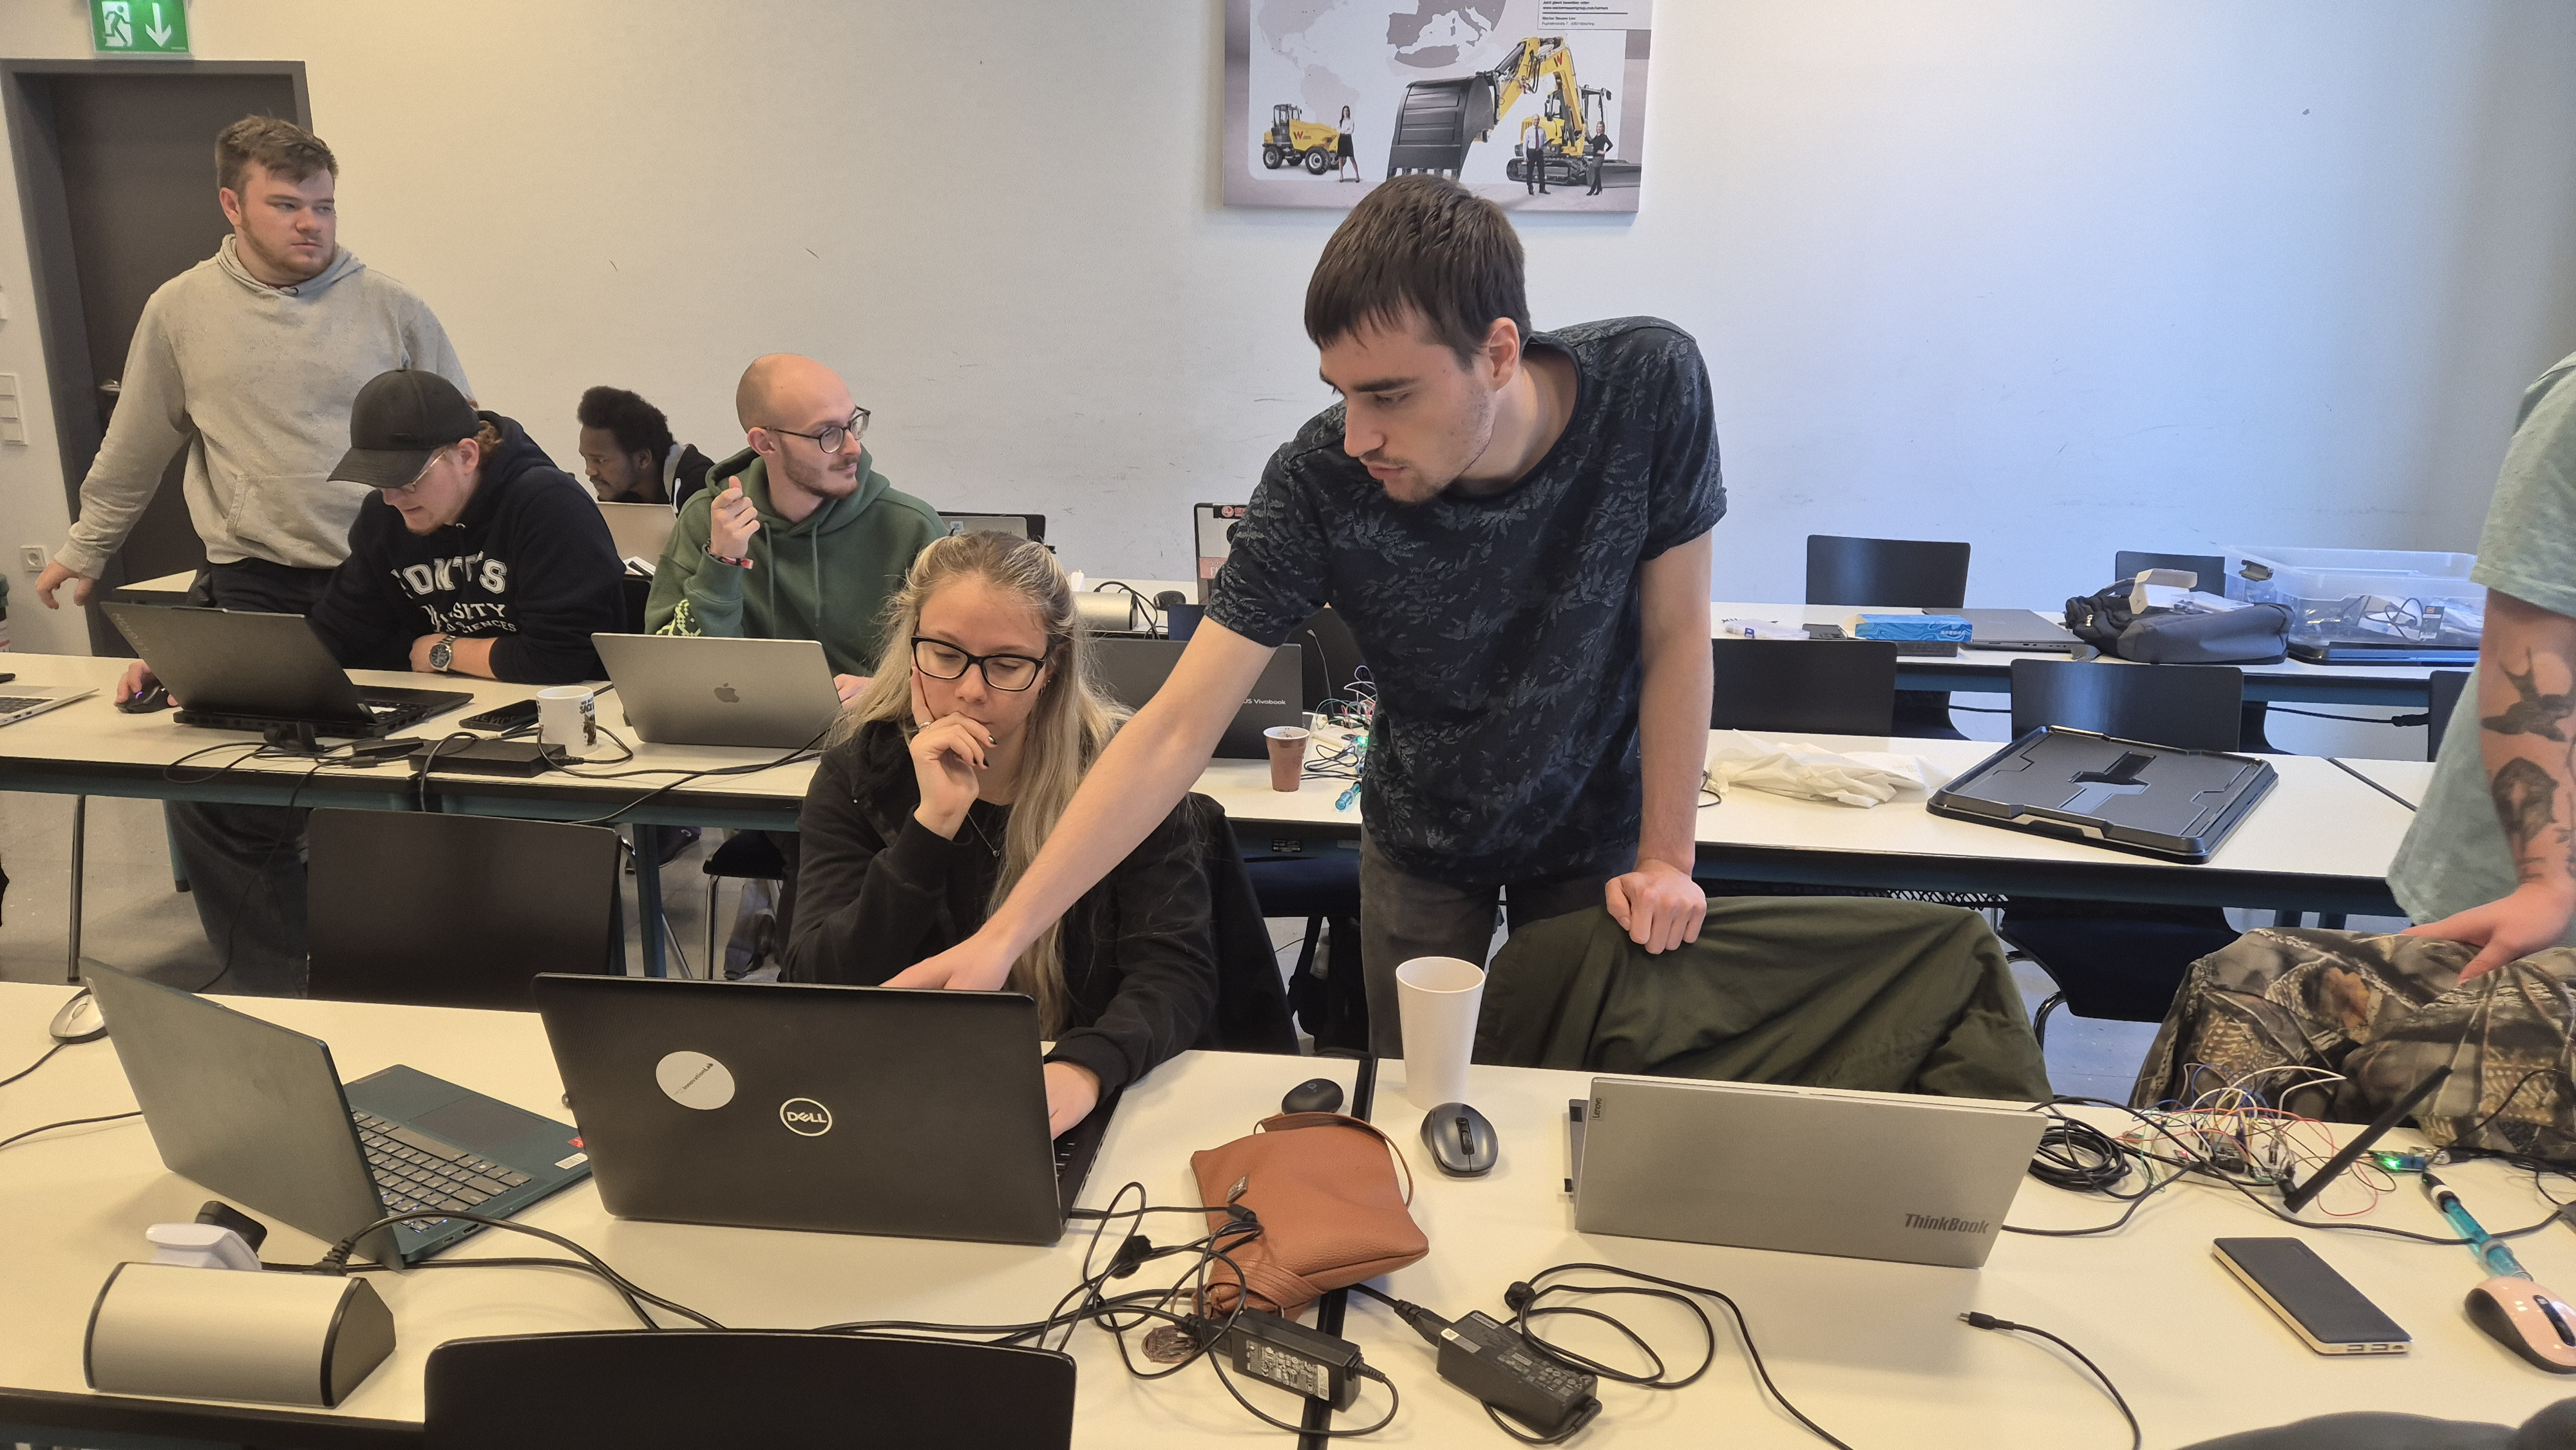
\includegraphics[width=\paperwidth,height=\paperheight,keepaspectratio]{material/B1}}%
\end{frame}
\begin{frame}[plain]
    \makebox[\linewidth]{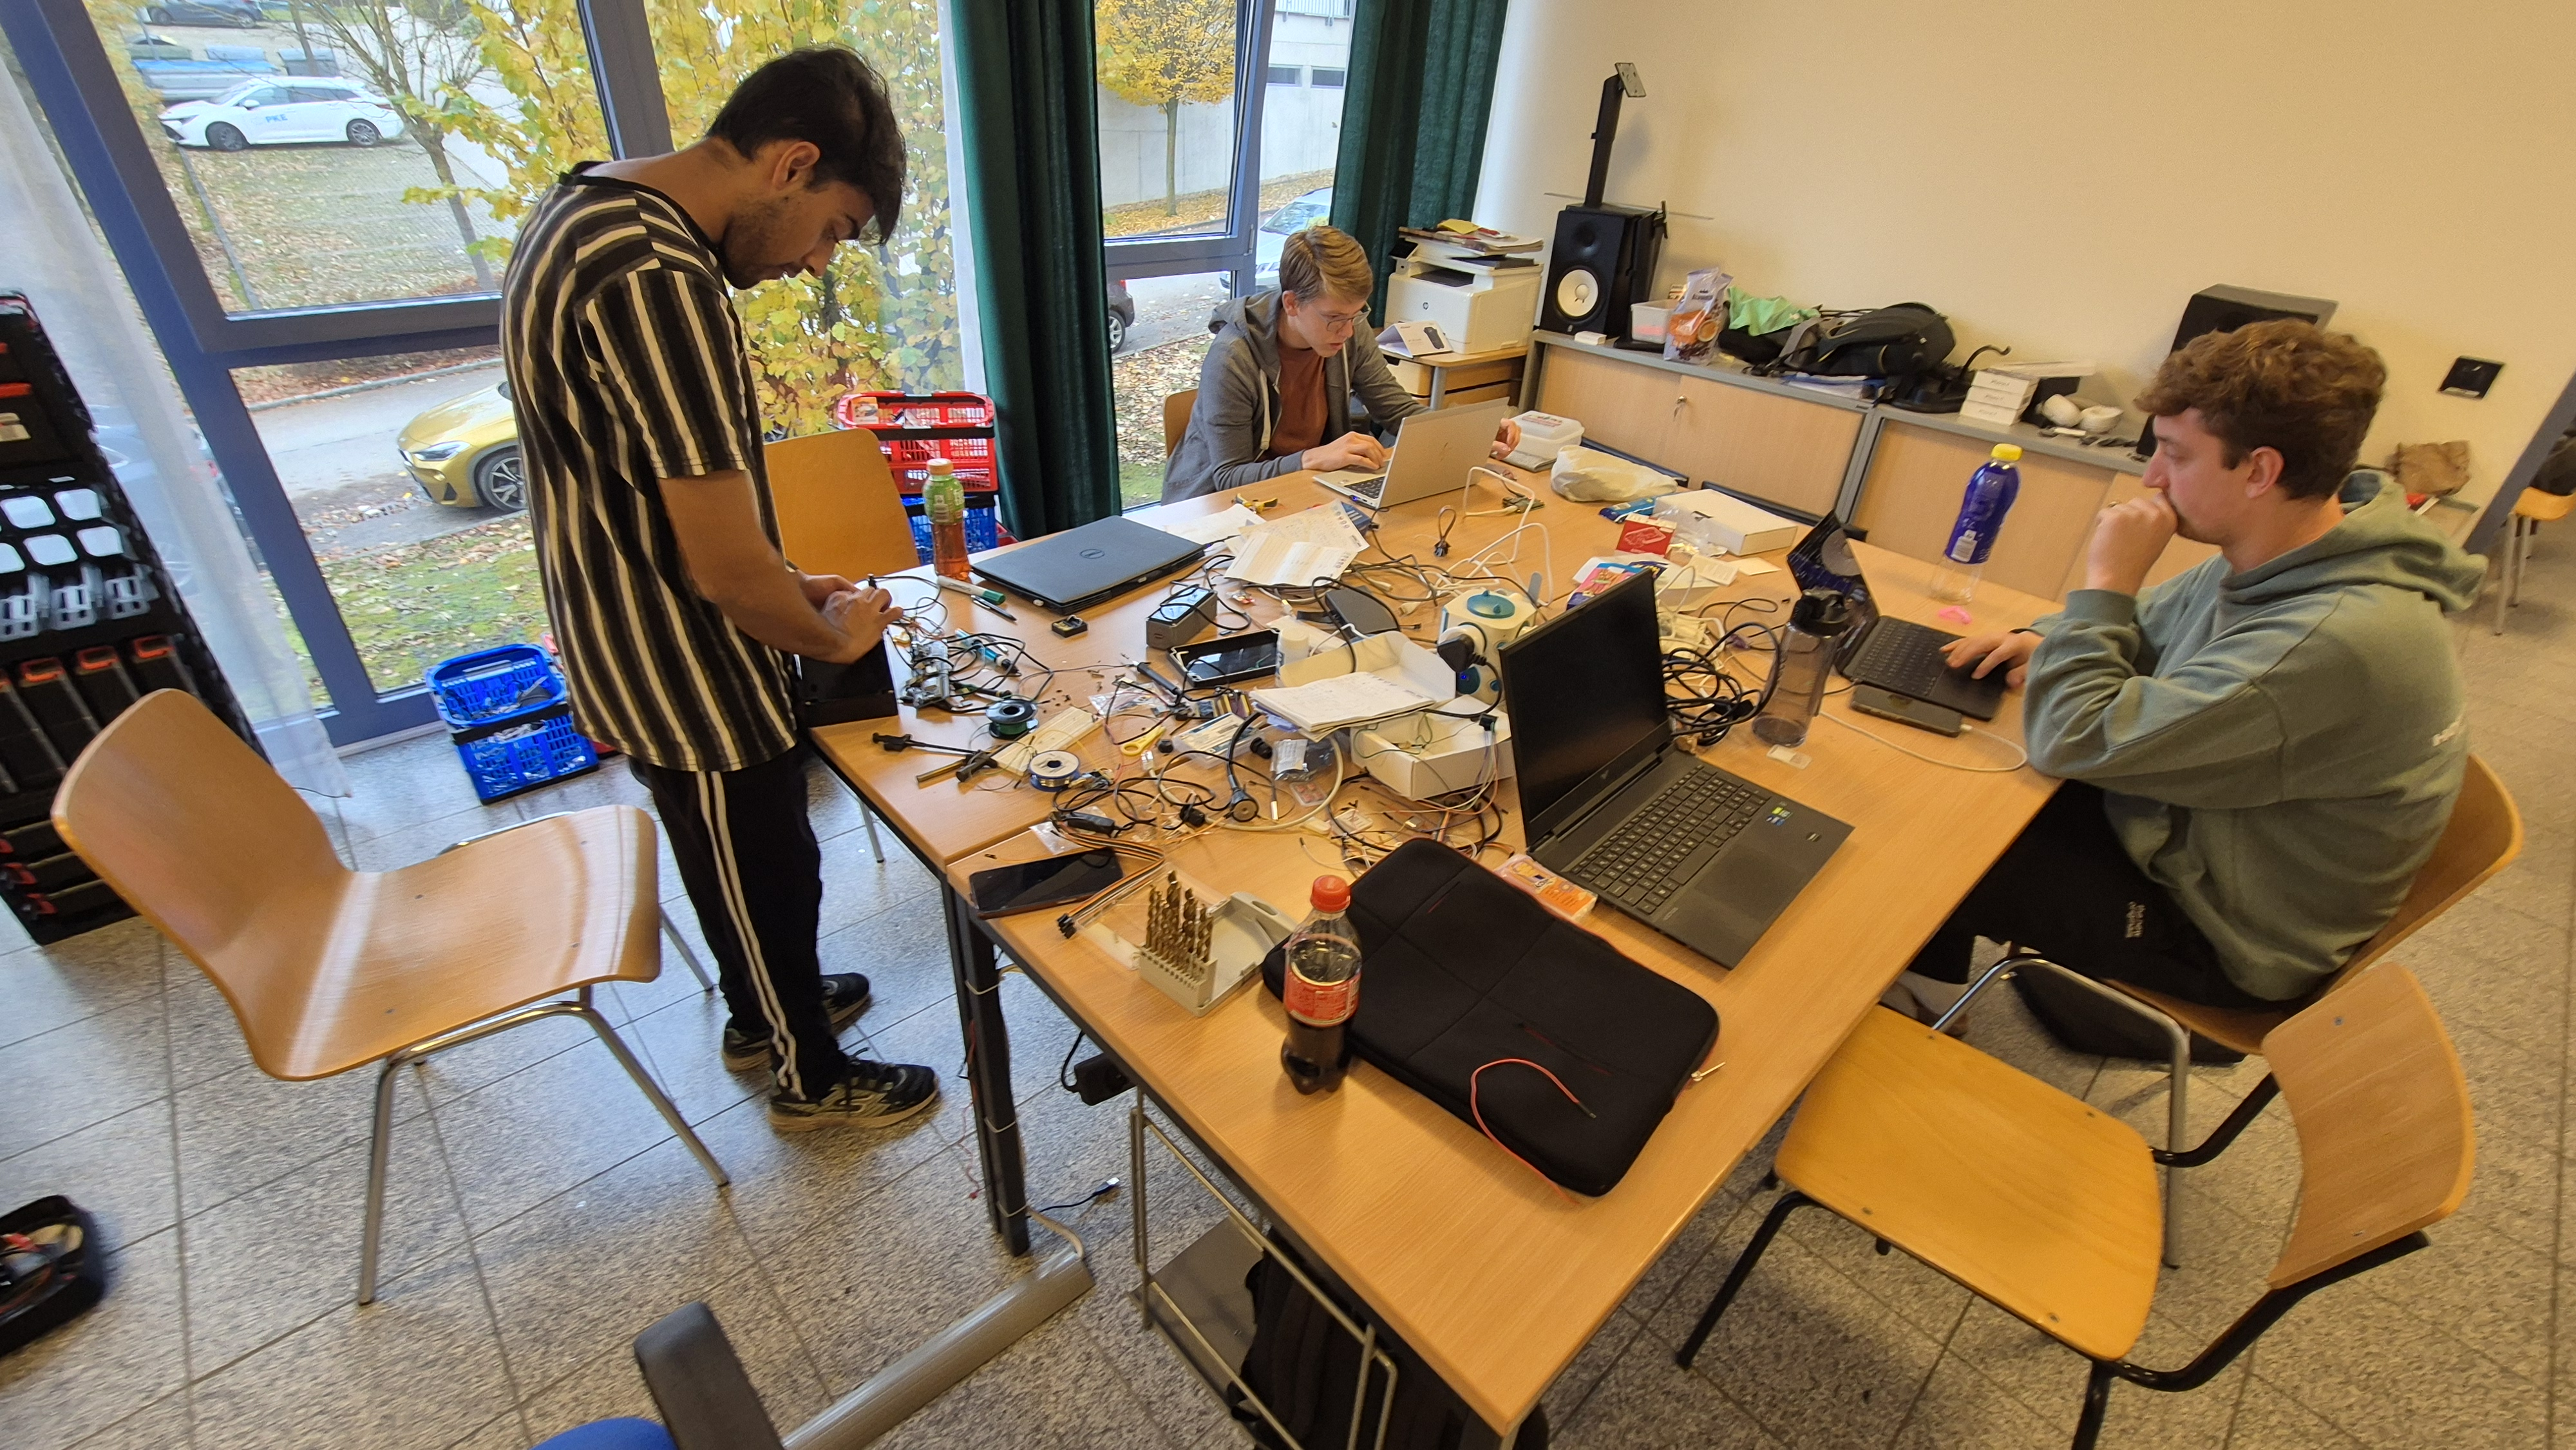
\includegraphics[width=\paperwidth,height=\paperheight,keepaspectratio]{material/C}}
\end{frame}
\begin{frame}[plain]
    \makebox[\linewidth]{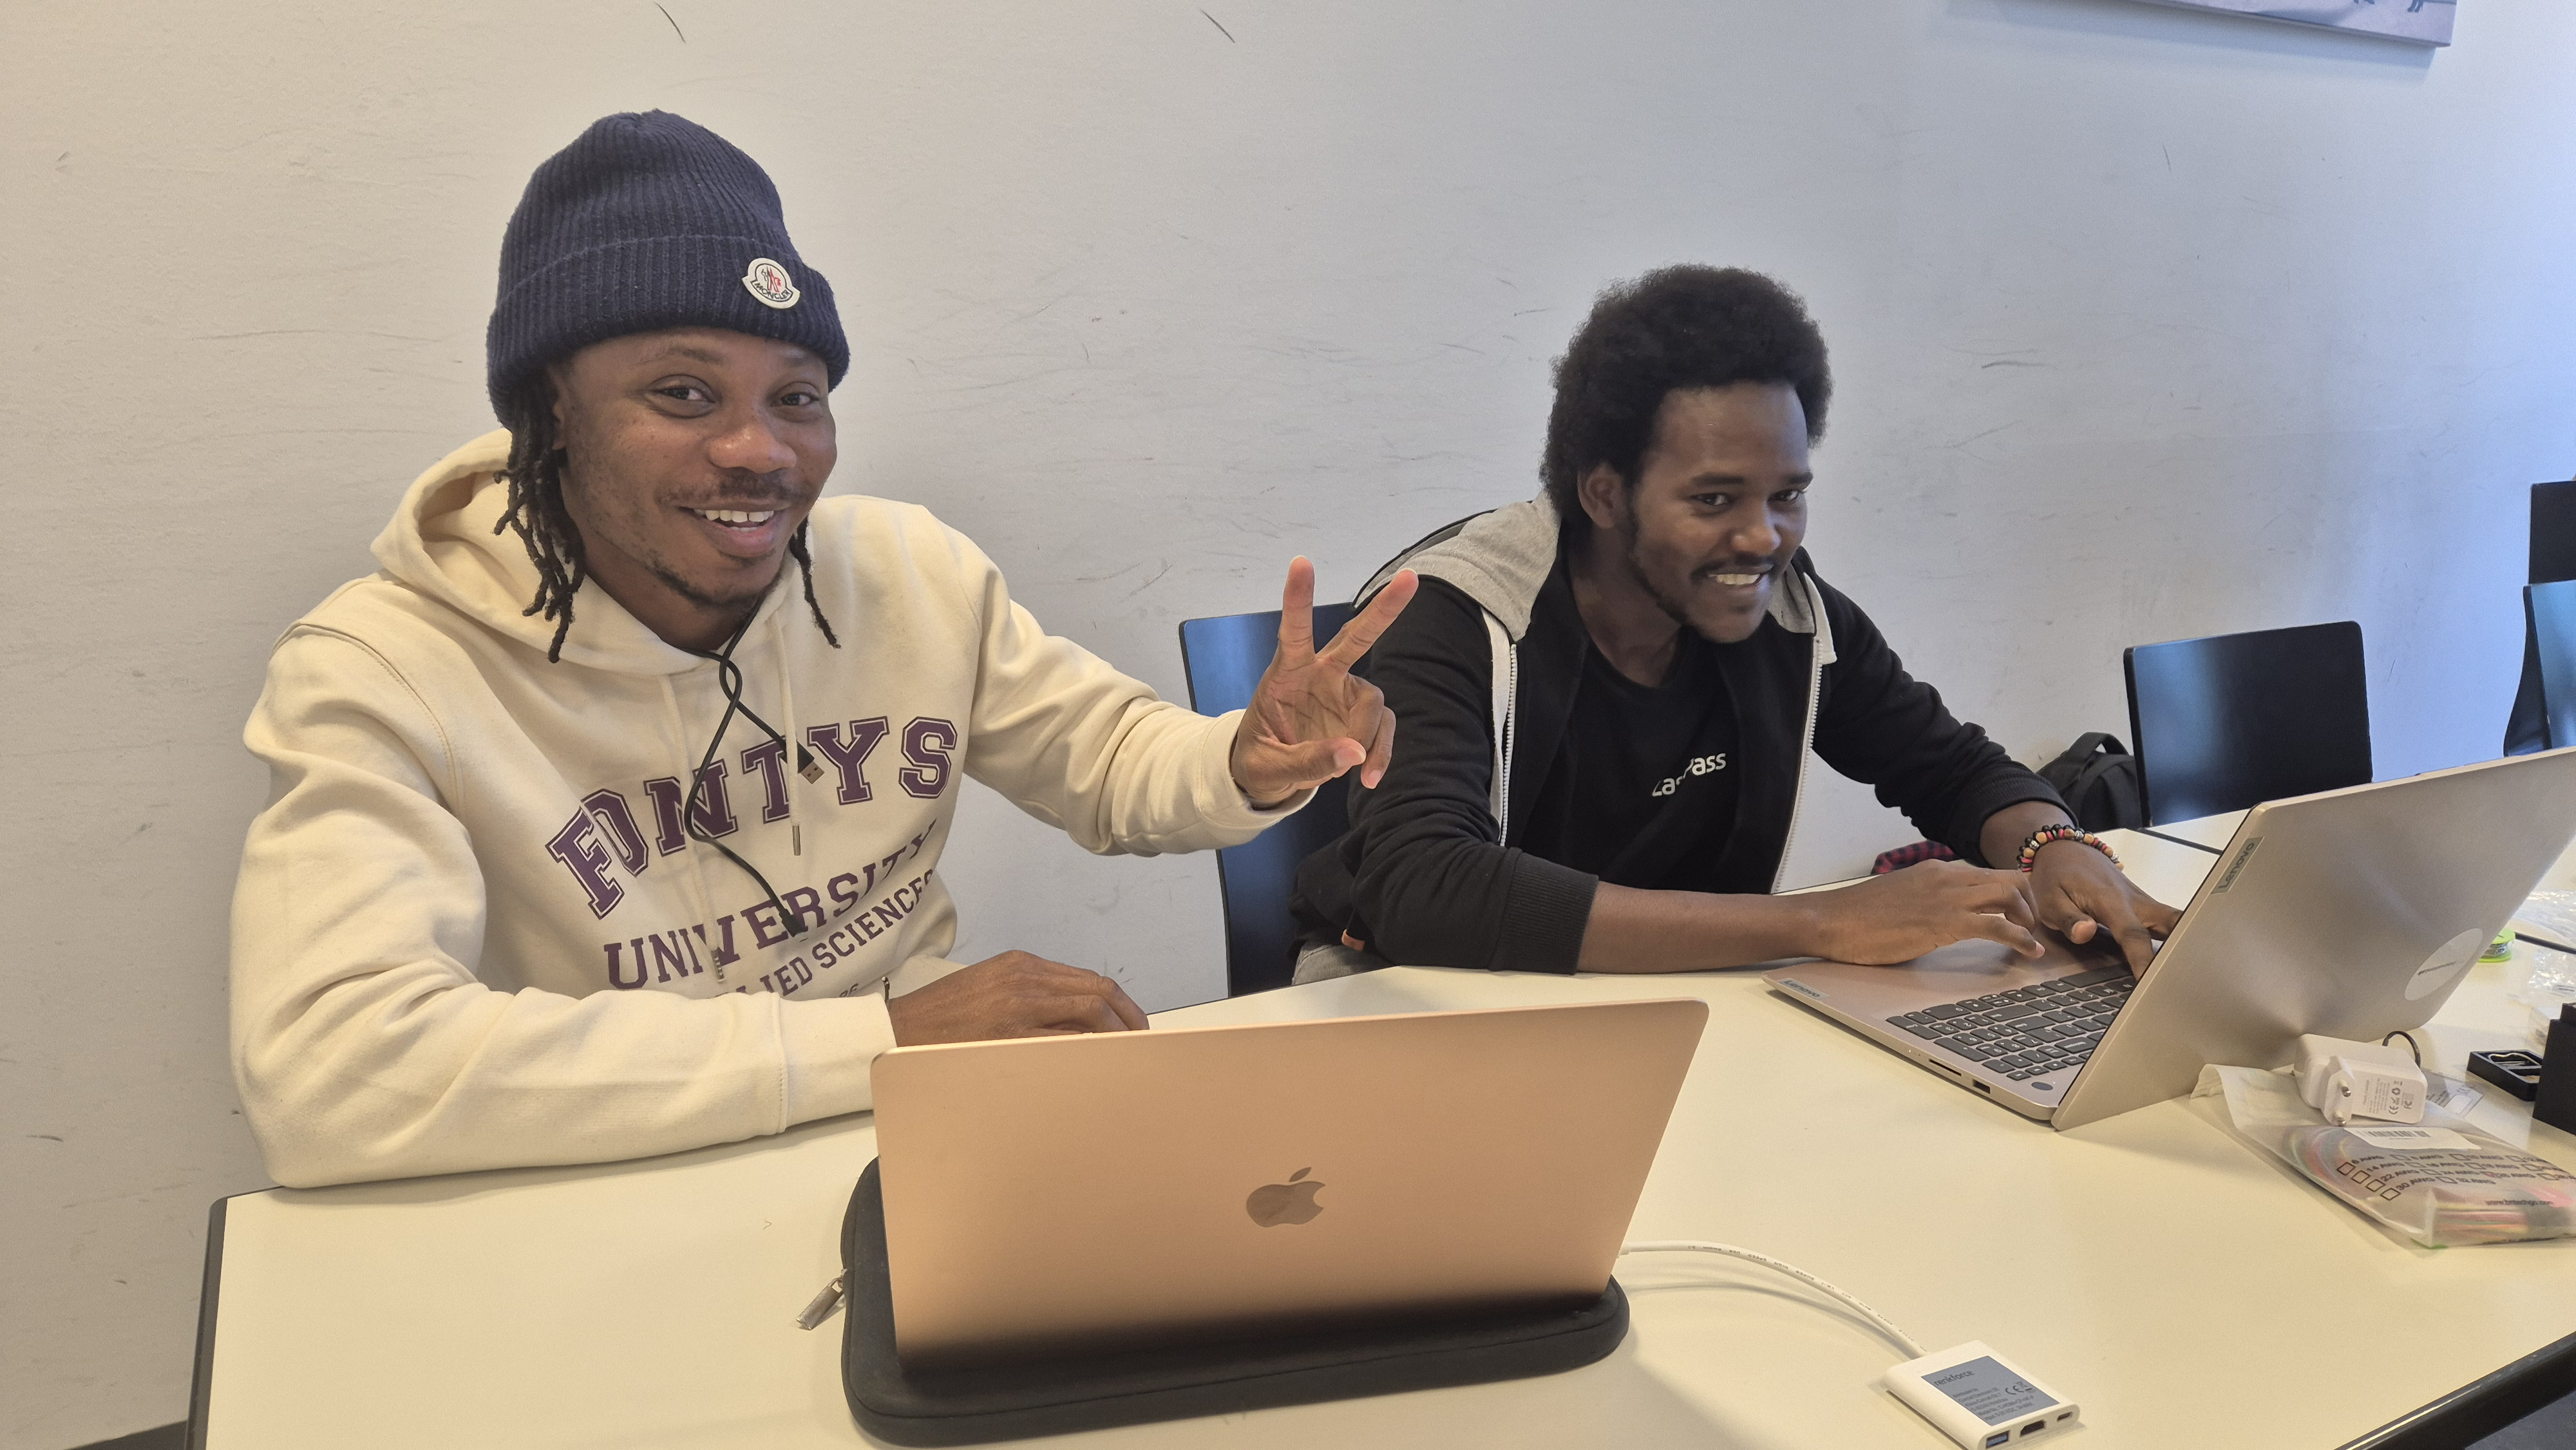
\includegraphics[width=\paperwidth,height=\paperheight,keepaspectratio]{material/C1}}
\end{frame}
\begin{frame}[plain]
    \makebox[\linewidth]{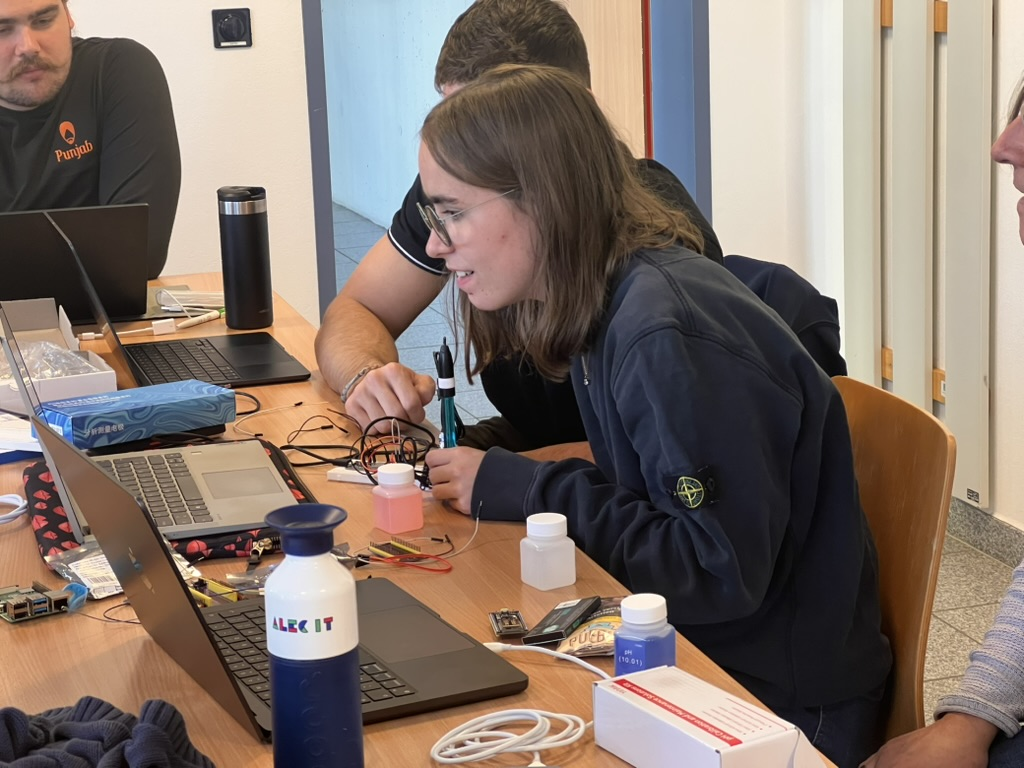
\includegraphics[width=\paperwidth,height=\paperheight,keepaspectratio]{material/D}}
\end{frame}
\begin{frame}[plain]
    \makebox[\linewidth]{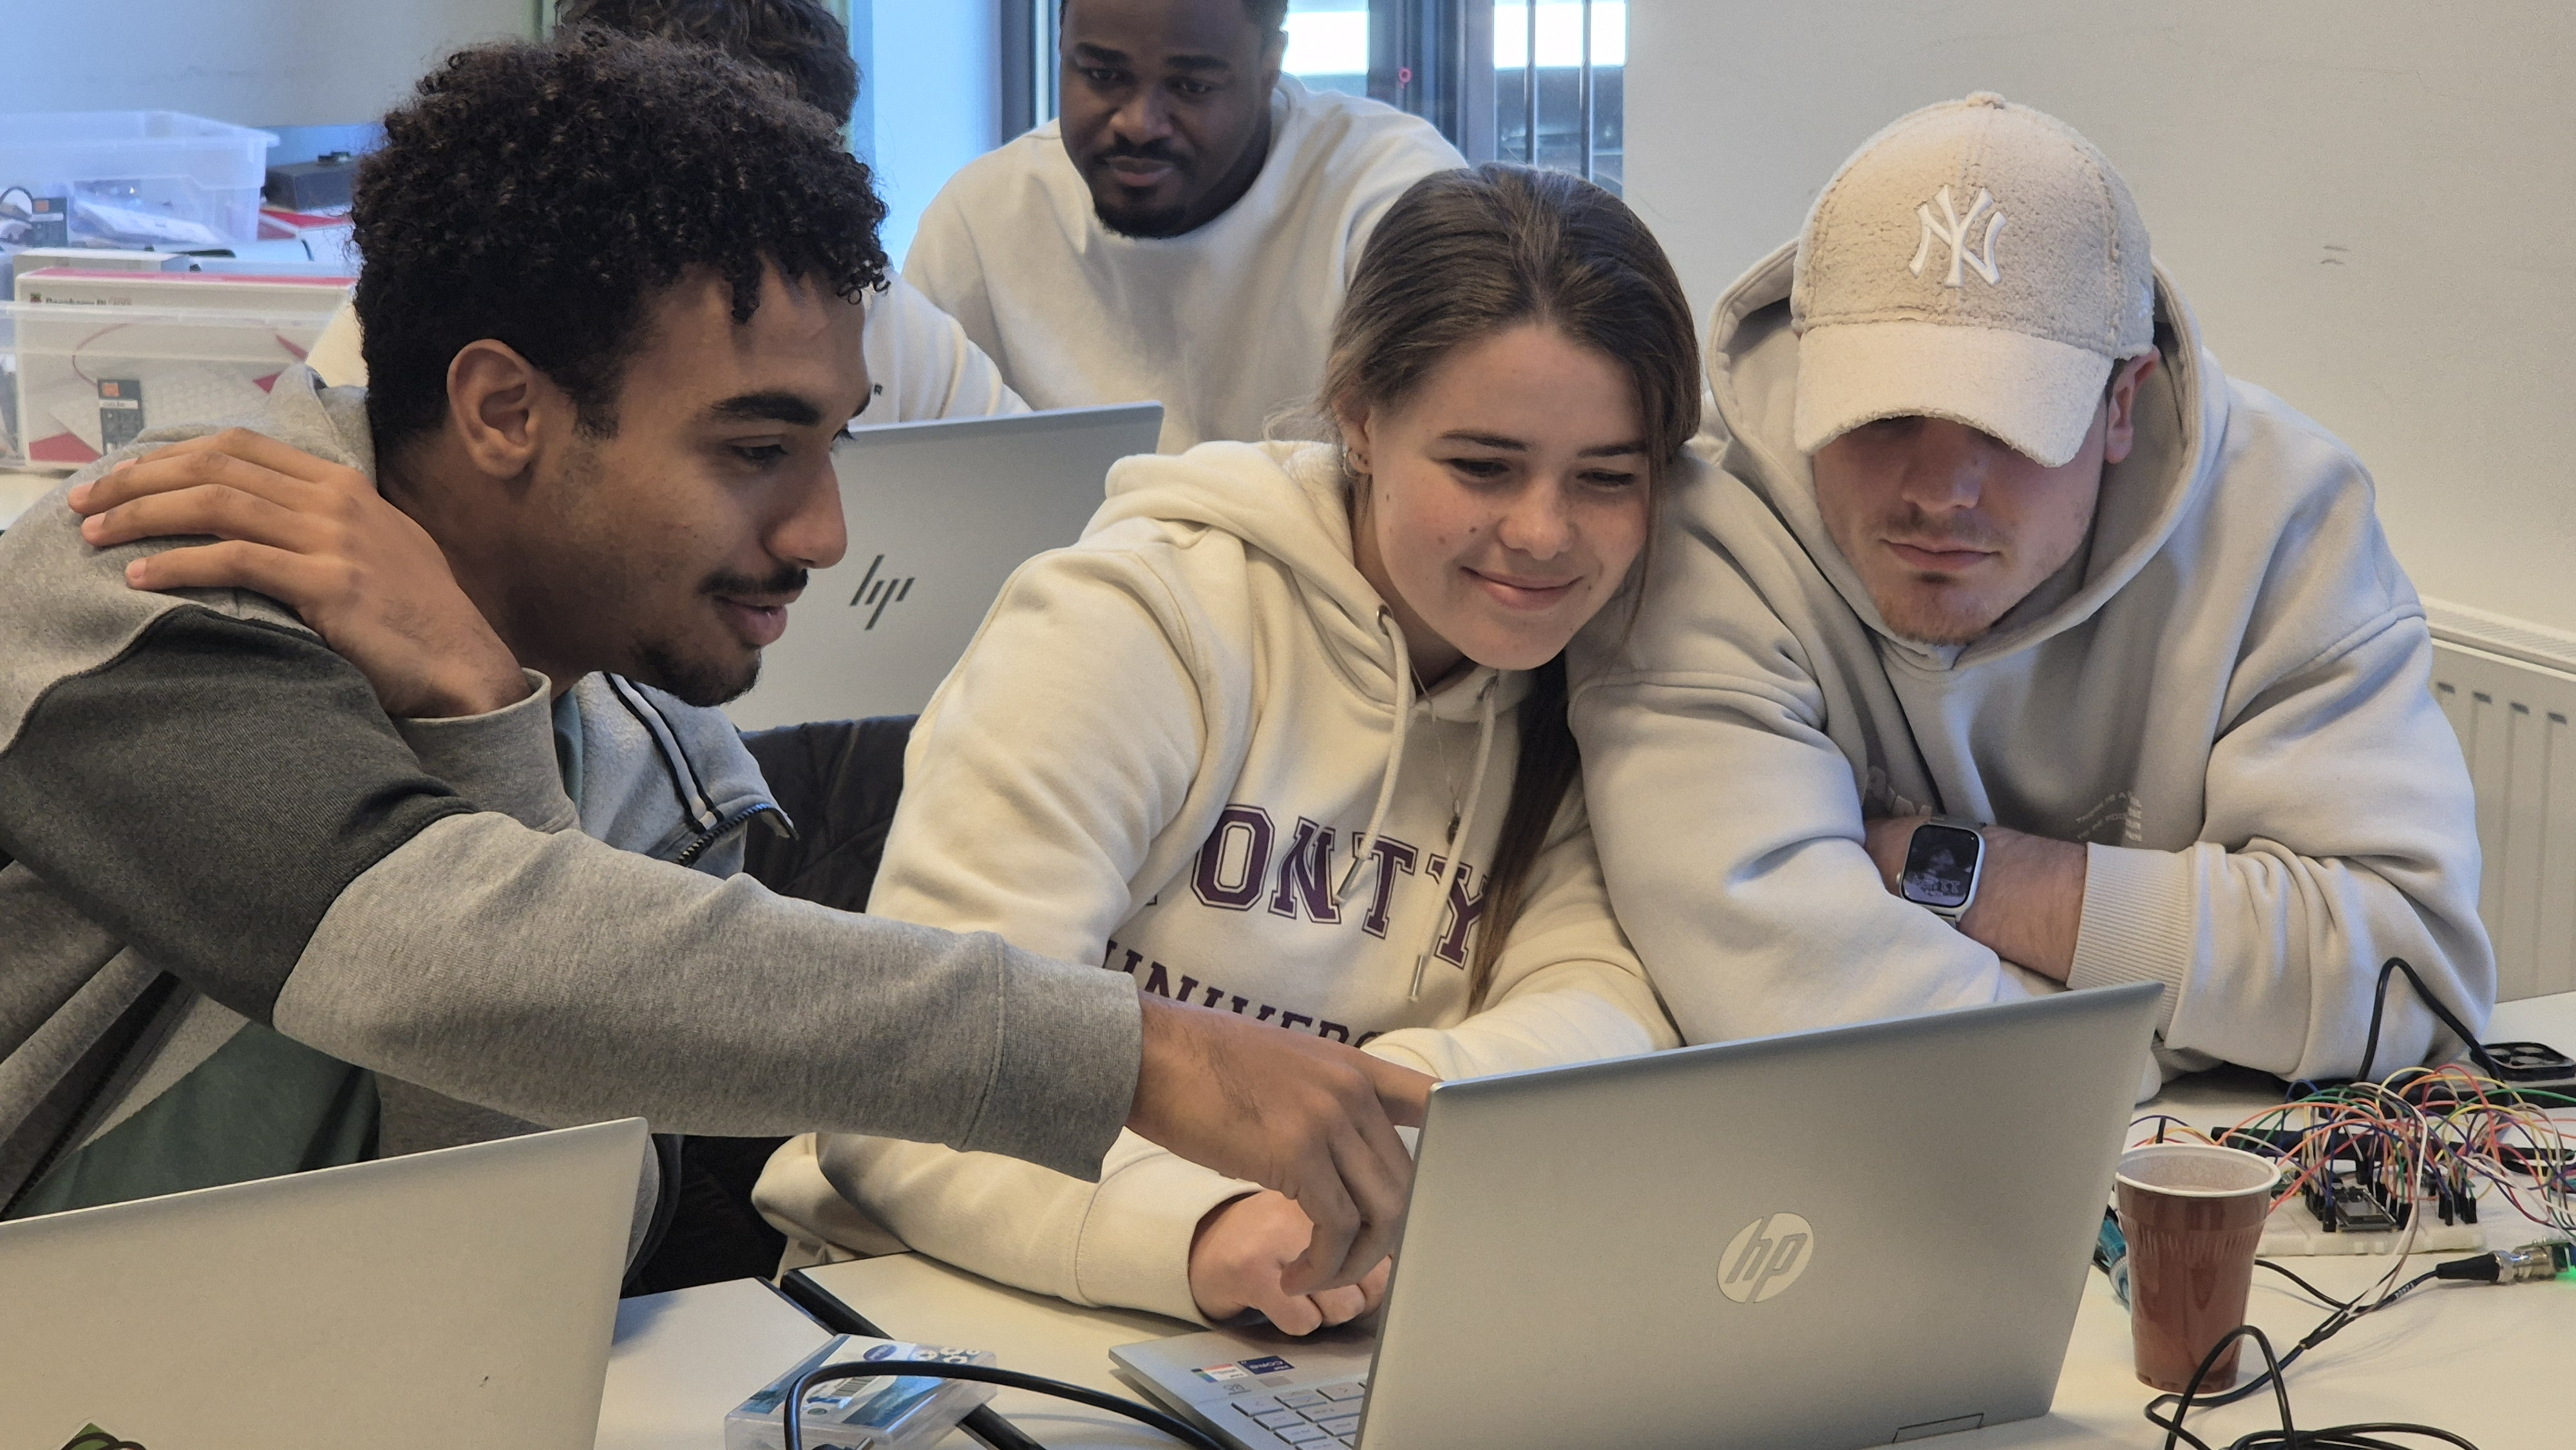
\includegraphics[width=\paperwidth,height=\paperheight,keepaspectratio]{material/D1}}
\end{frame}
\begin{frame}[plain]
    \makebox[\linewidth]{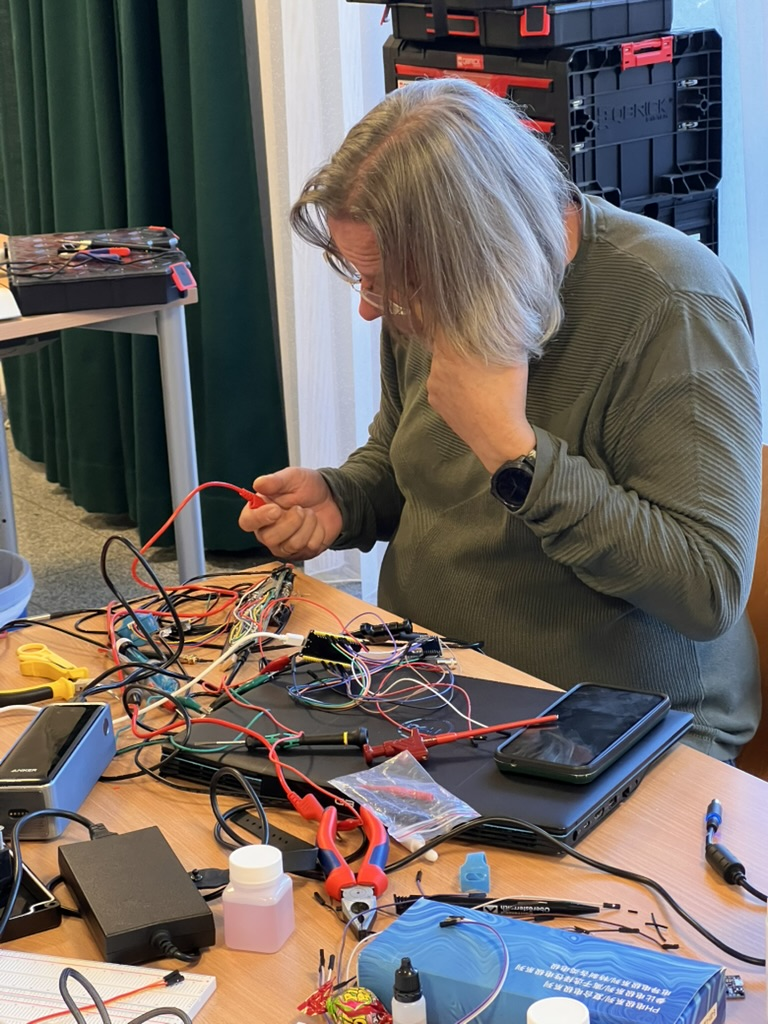
\includegraphics[width=\paperwidth,height=\paperheight,keepaspectratio]{material/E}}
\end{frame}
\begin{frame}[plain]
    \makebox[\linewidth]{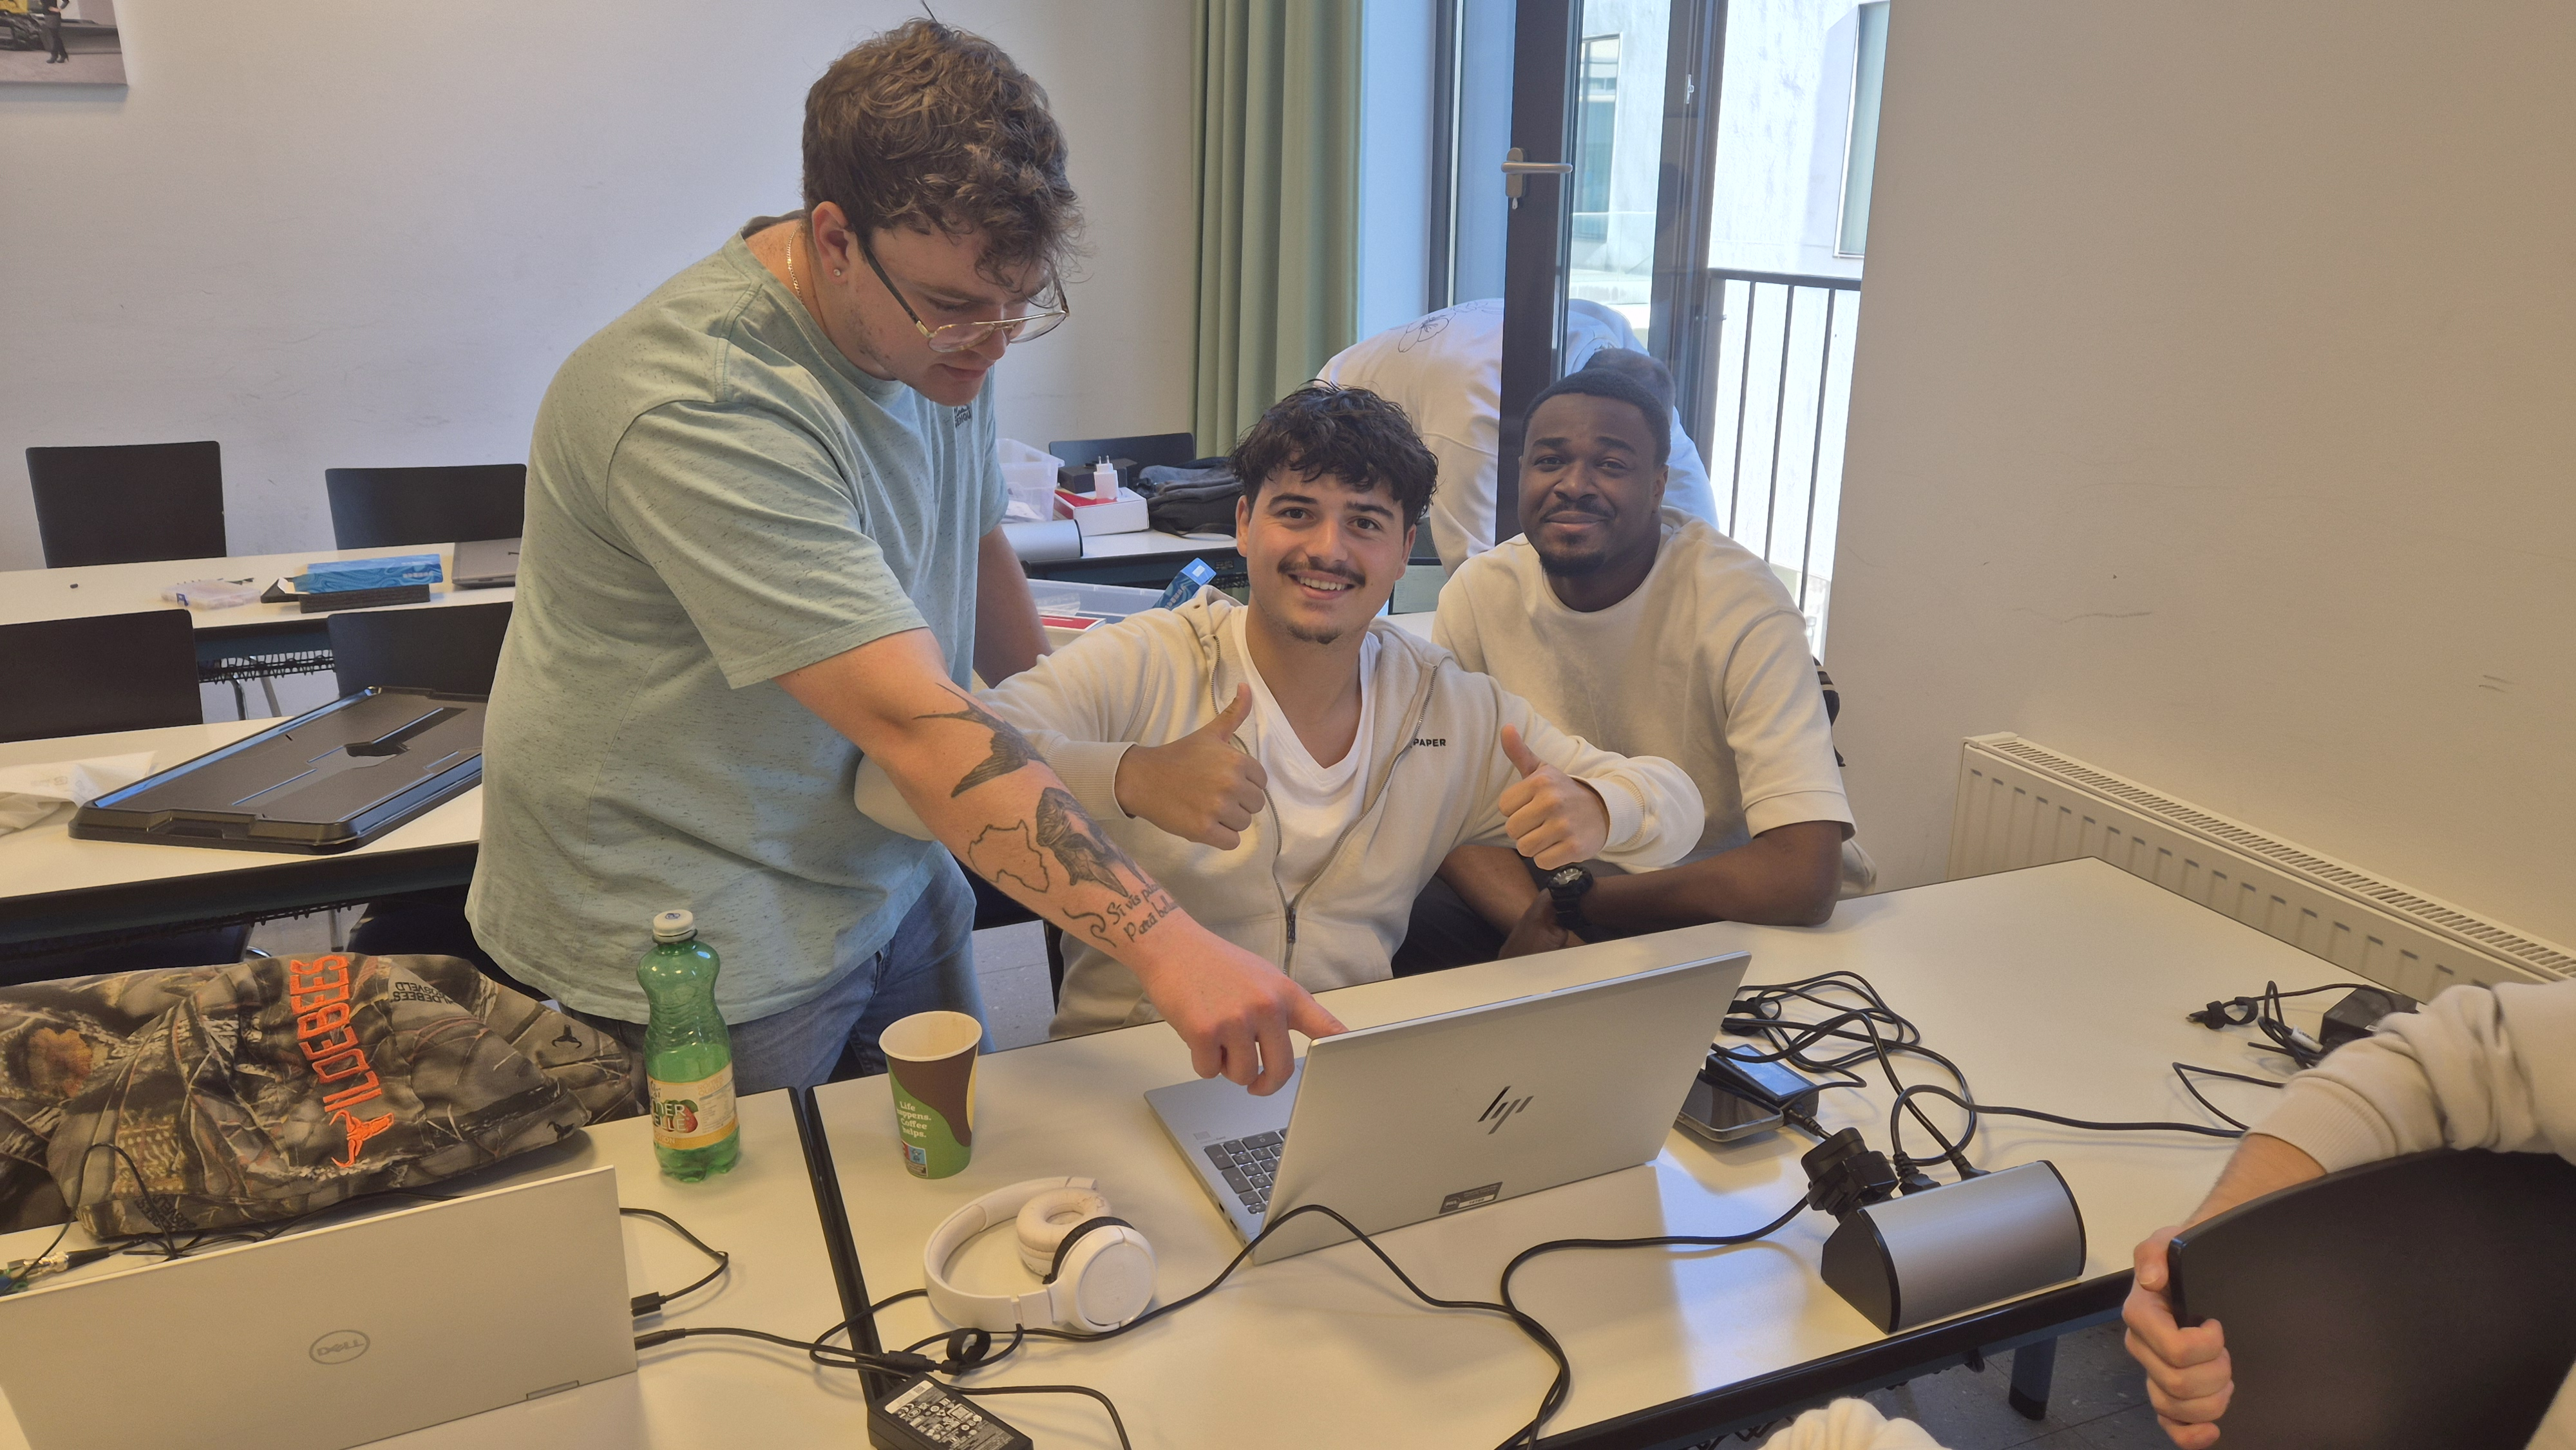
\includegraphics[width=\paperwidth,height=\paperheight,keepaspectratio]{material/E1}}
\end{frame}
\begin{frame}[plain]
    \makebox[\linewidth]{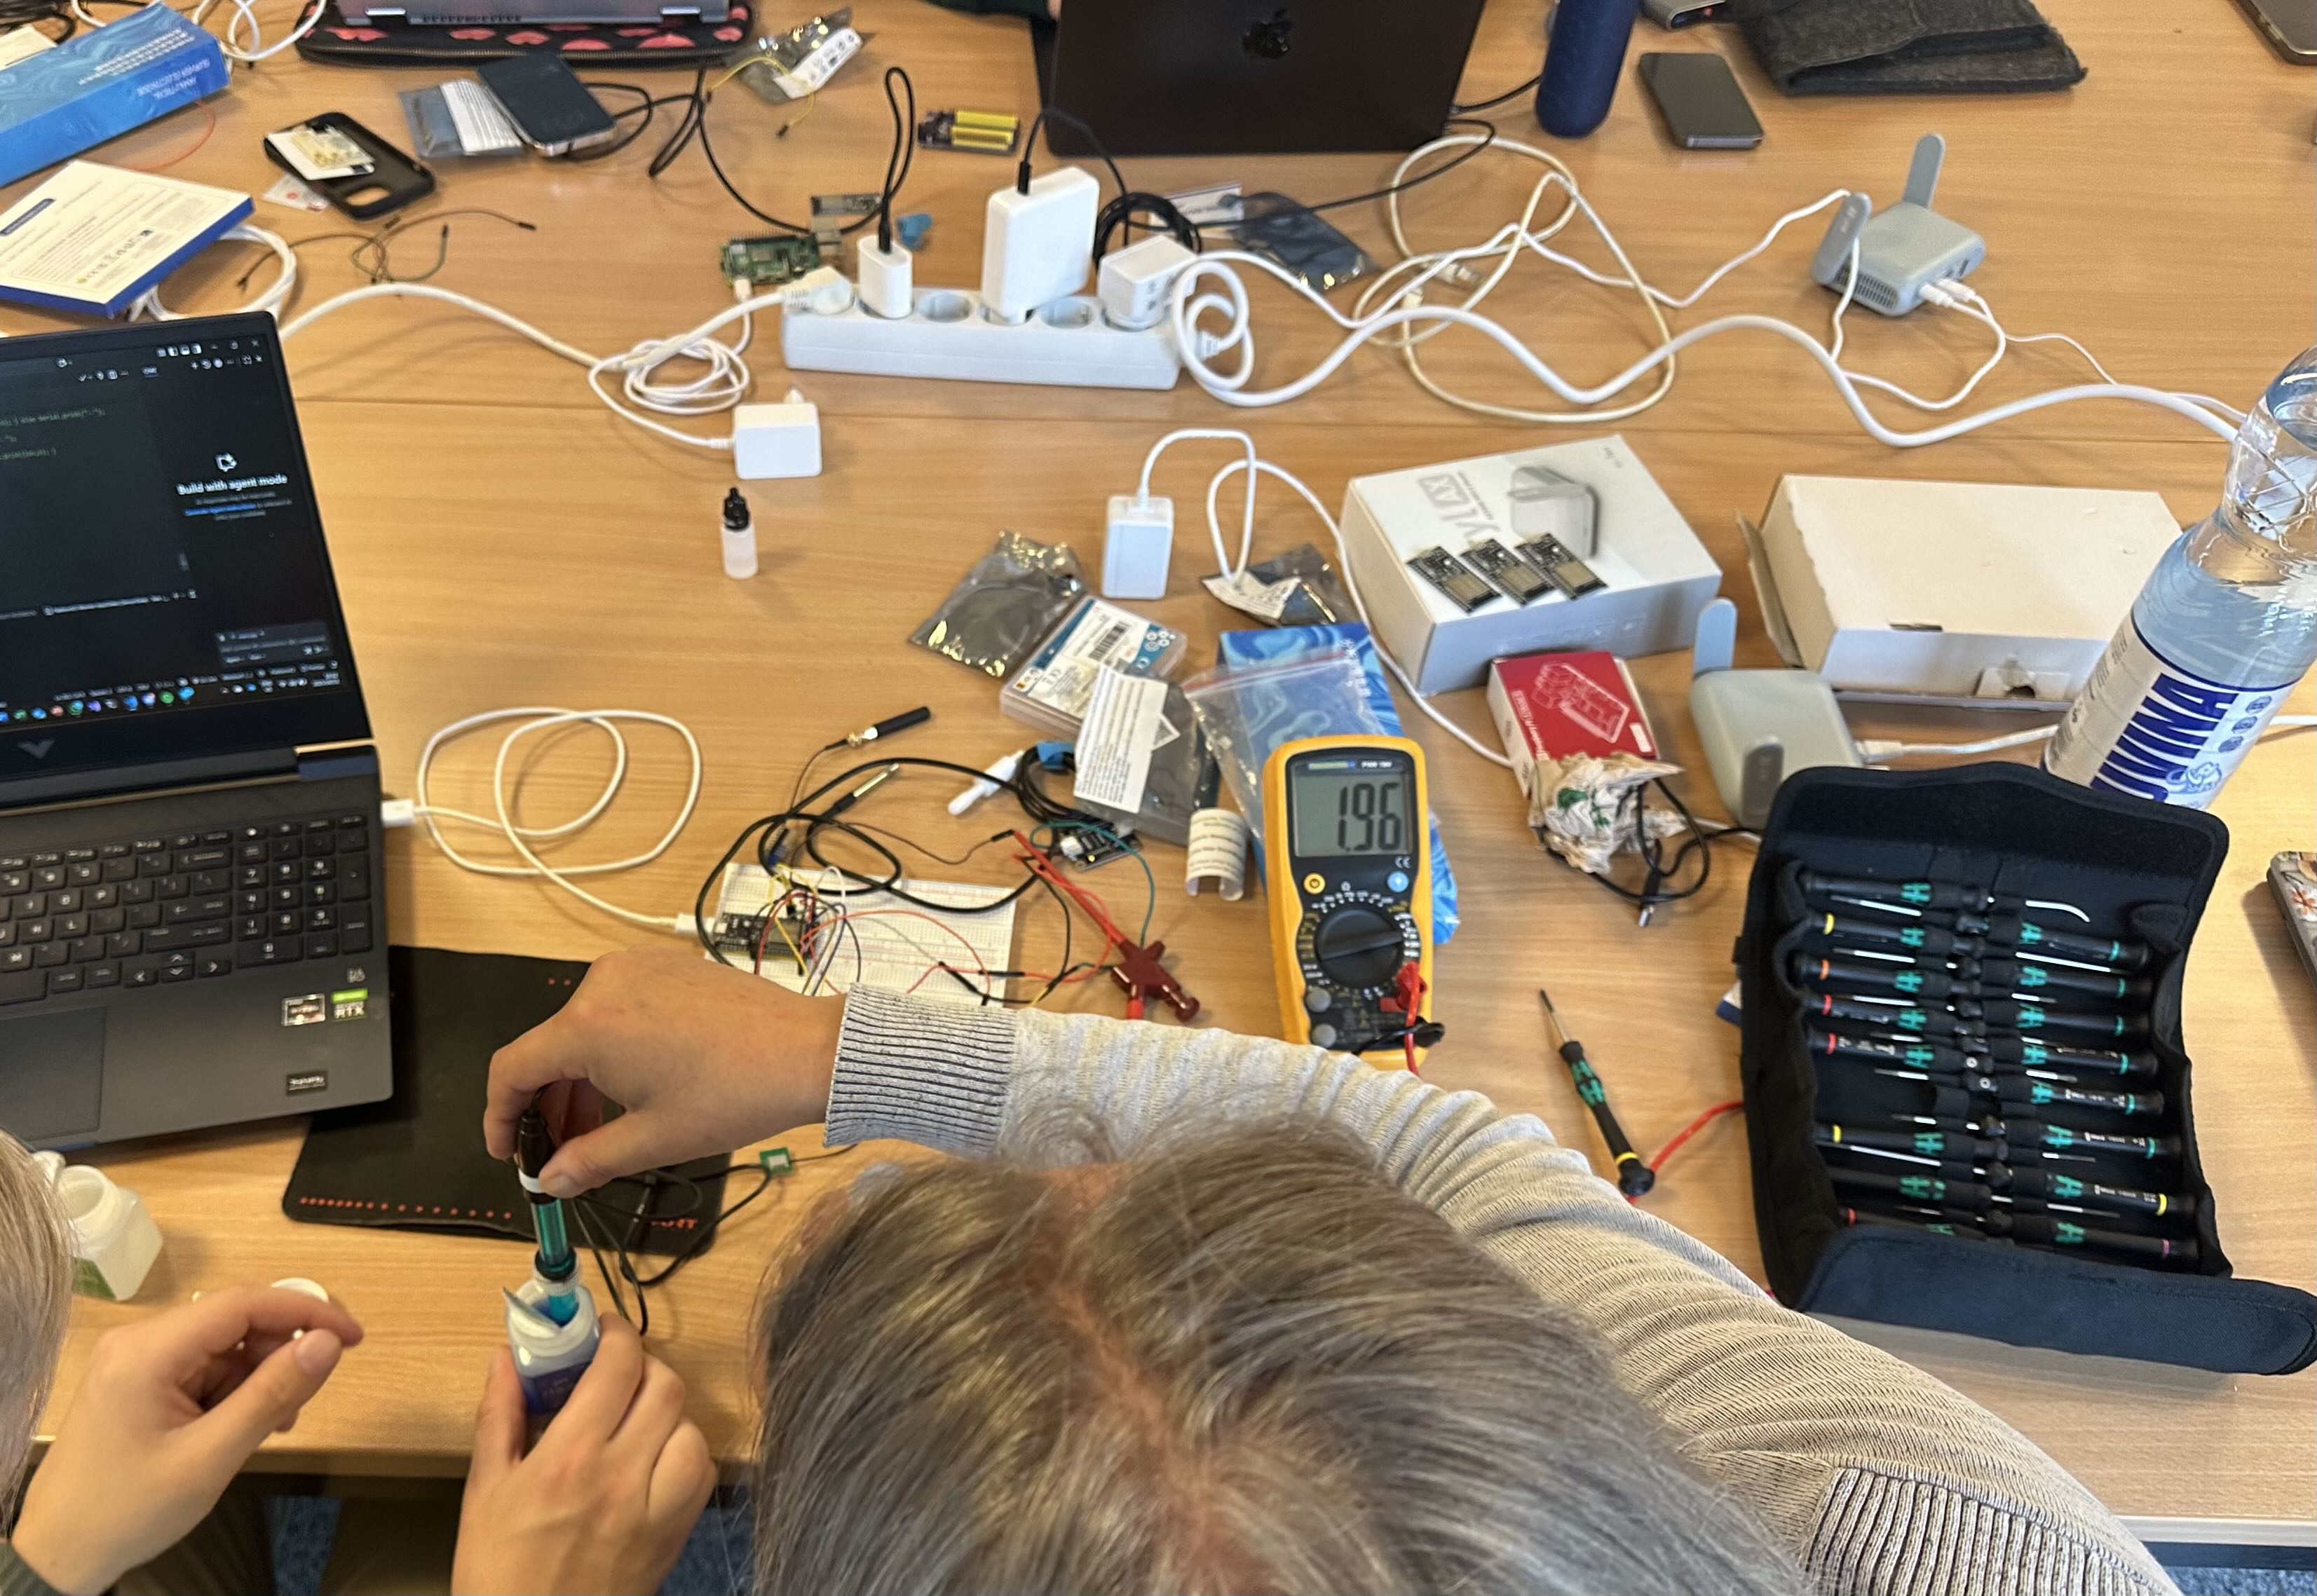
\includegraphics[width=\paperwidth,height=\paperheight,keepaspectratio]{material/F}}
\end{frame}
\begin{frame}[plain]
    \makebox[\linewidth]{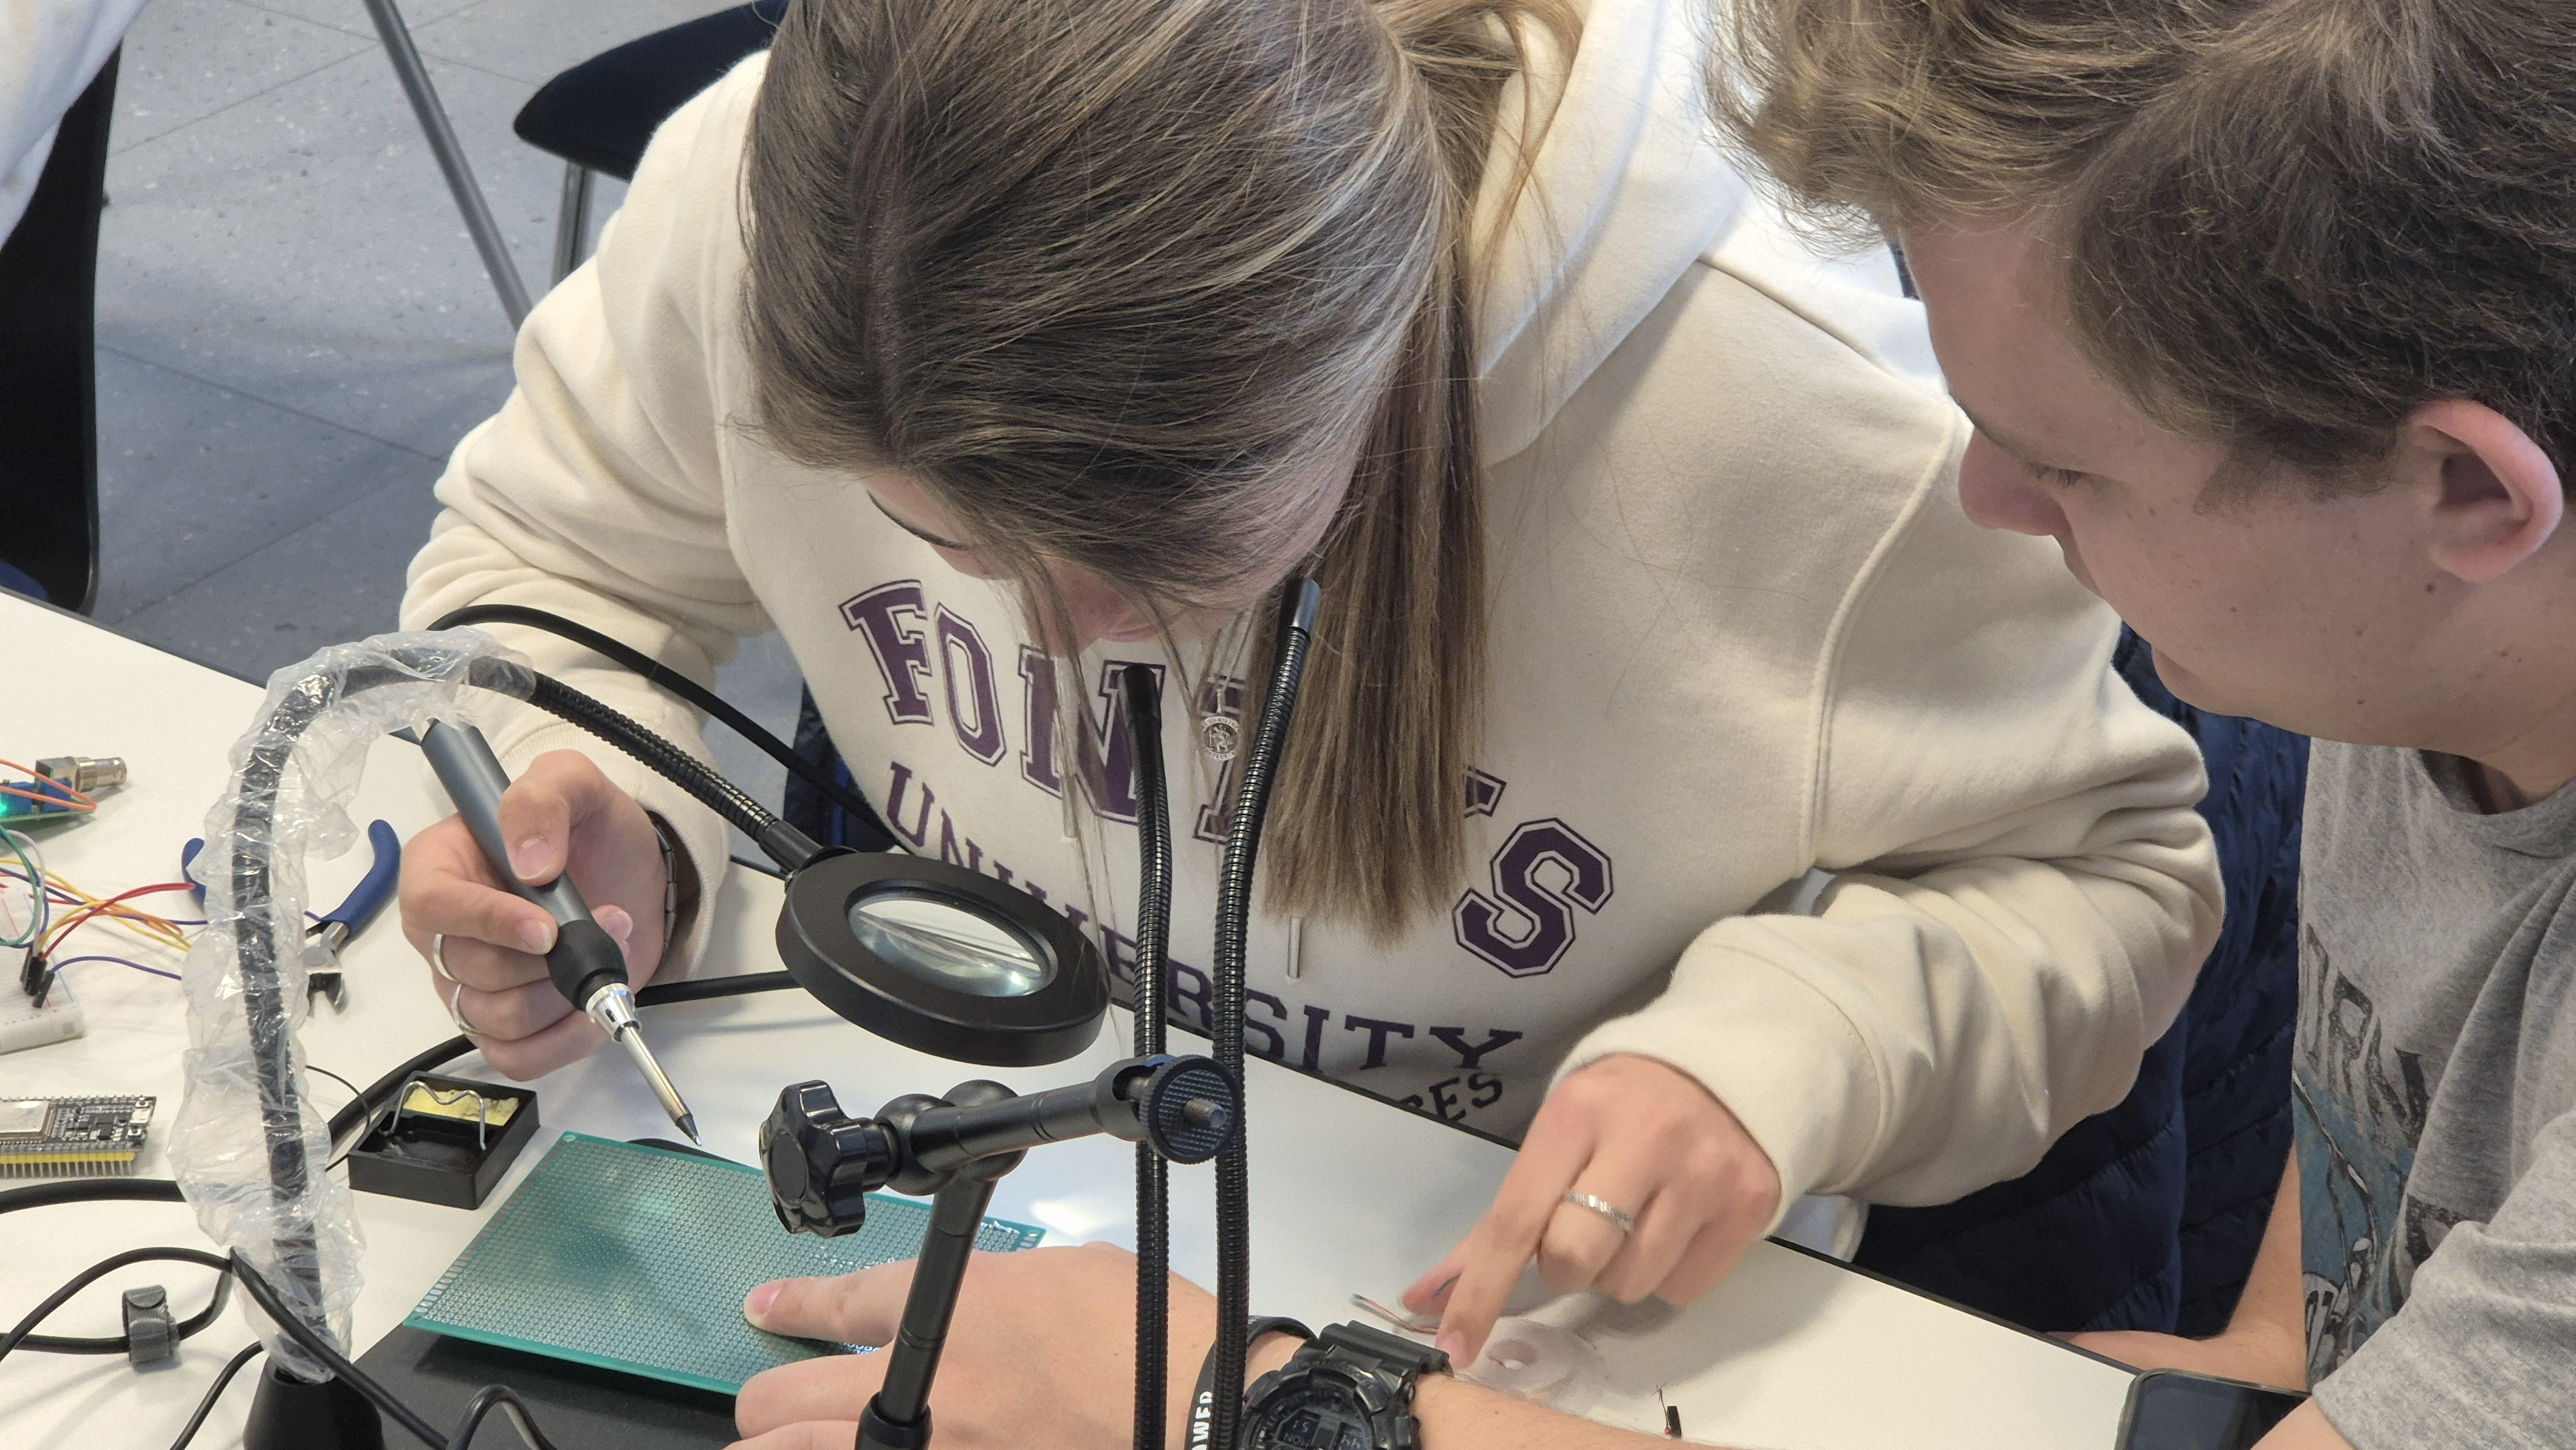
\includegraphics[width=\paperwidth,height=\paperheight,keepaspectratio]{material/F1}}
\end{frame}
\begin{frame}[plain]
    \makebox[\linewidth]{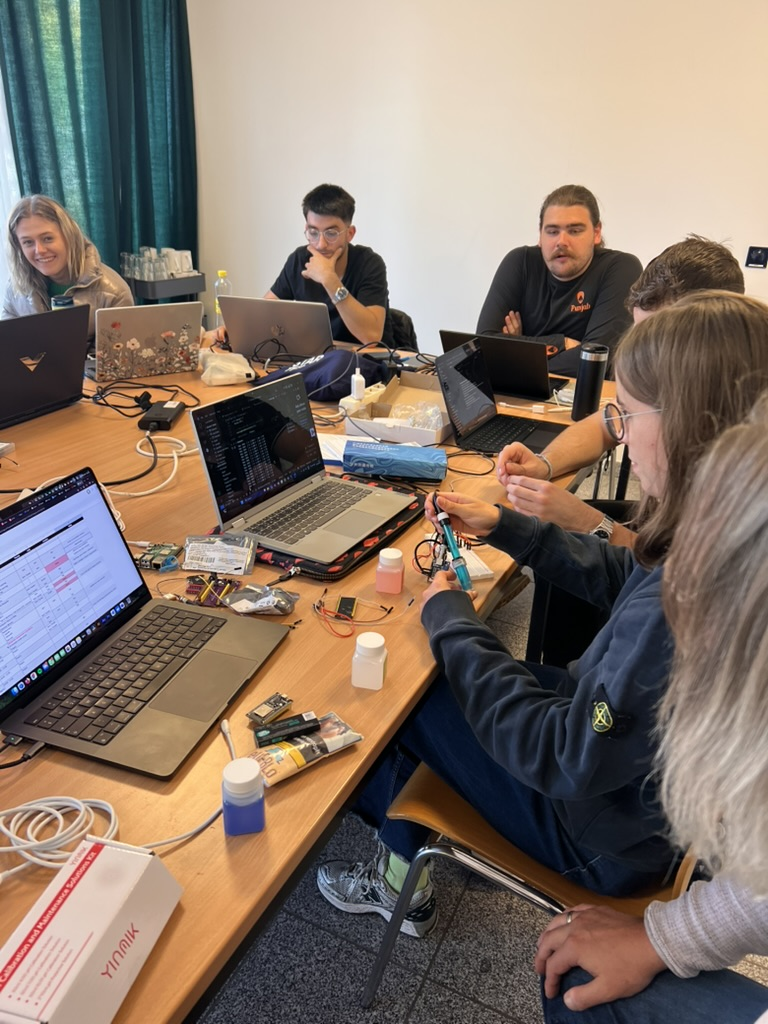
\includegraphics[width=\paperwidth,height=\paperheight,keepaspectratio]{material/G}}
\end{frame}
\begin{frame}[plain]
    \makebox[\linewidth]{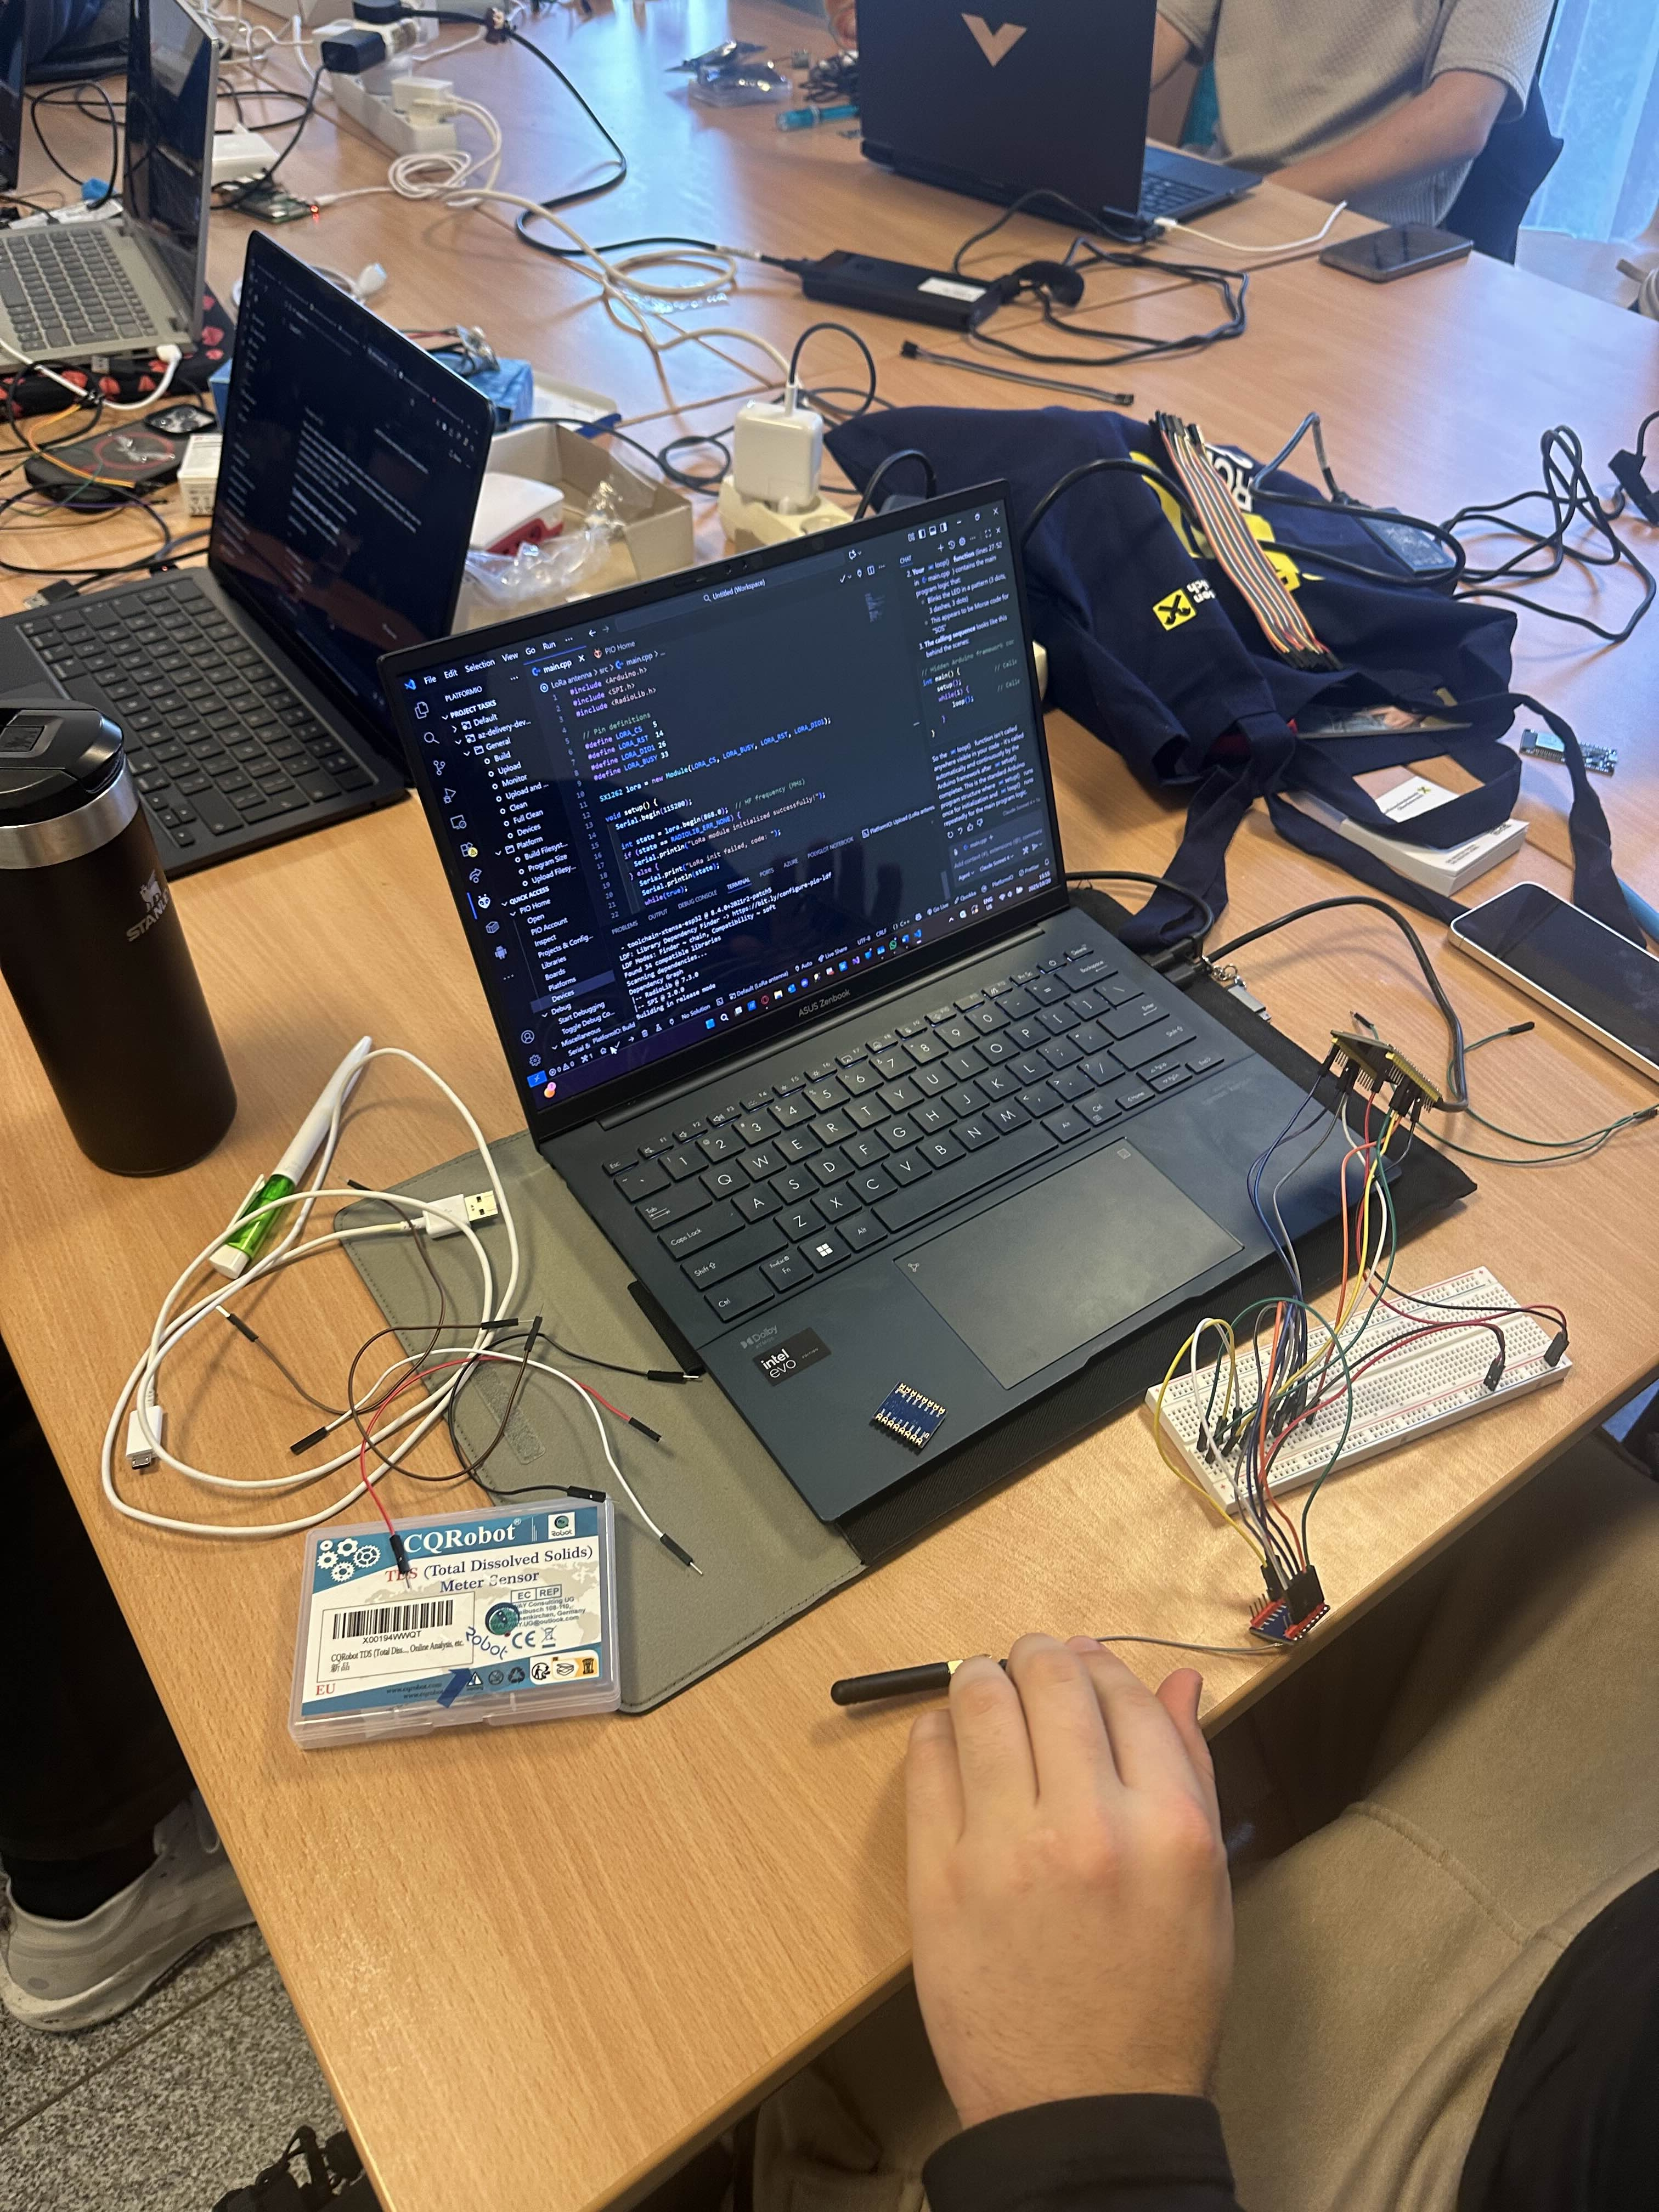
\includegraphics[width=\paperwidth,height=\paperheight,keepaspectratio]{material/H}}
\end{frame}
\begin{frame}[plain]
    \makebox[\linewidth]{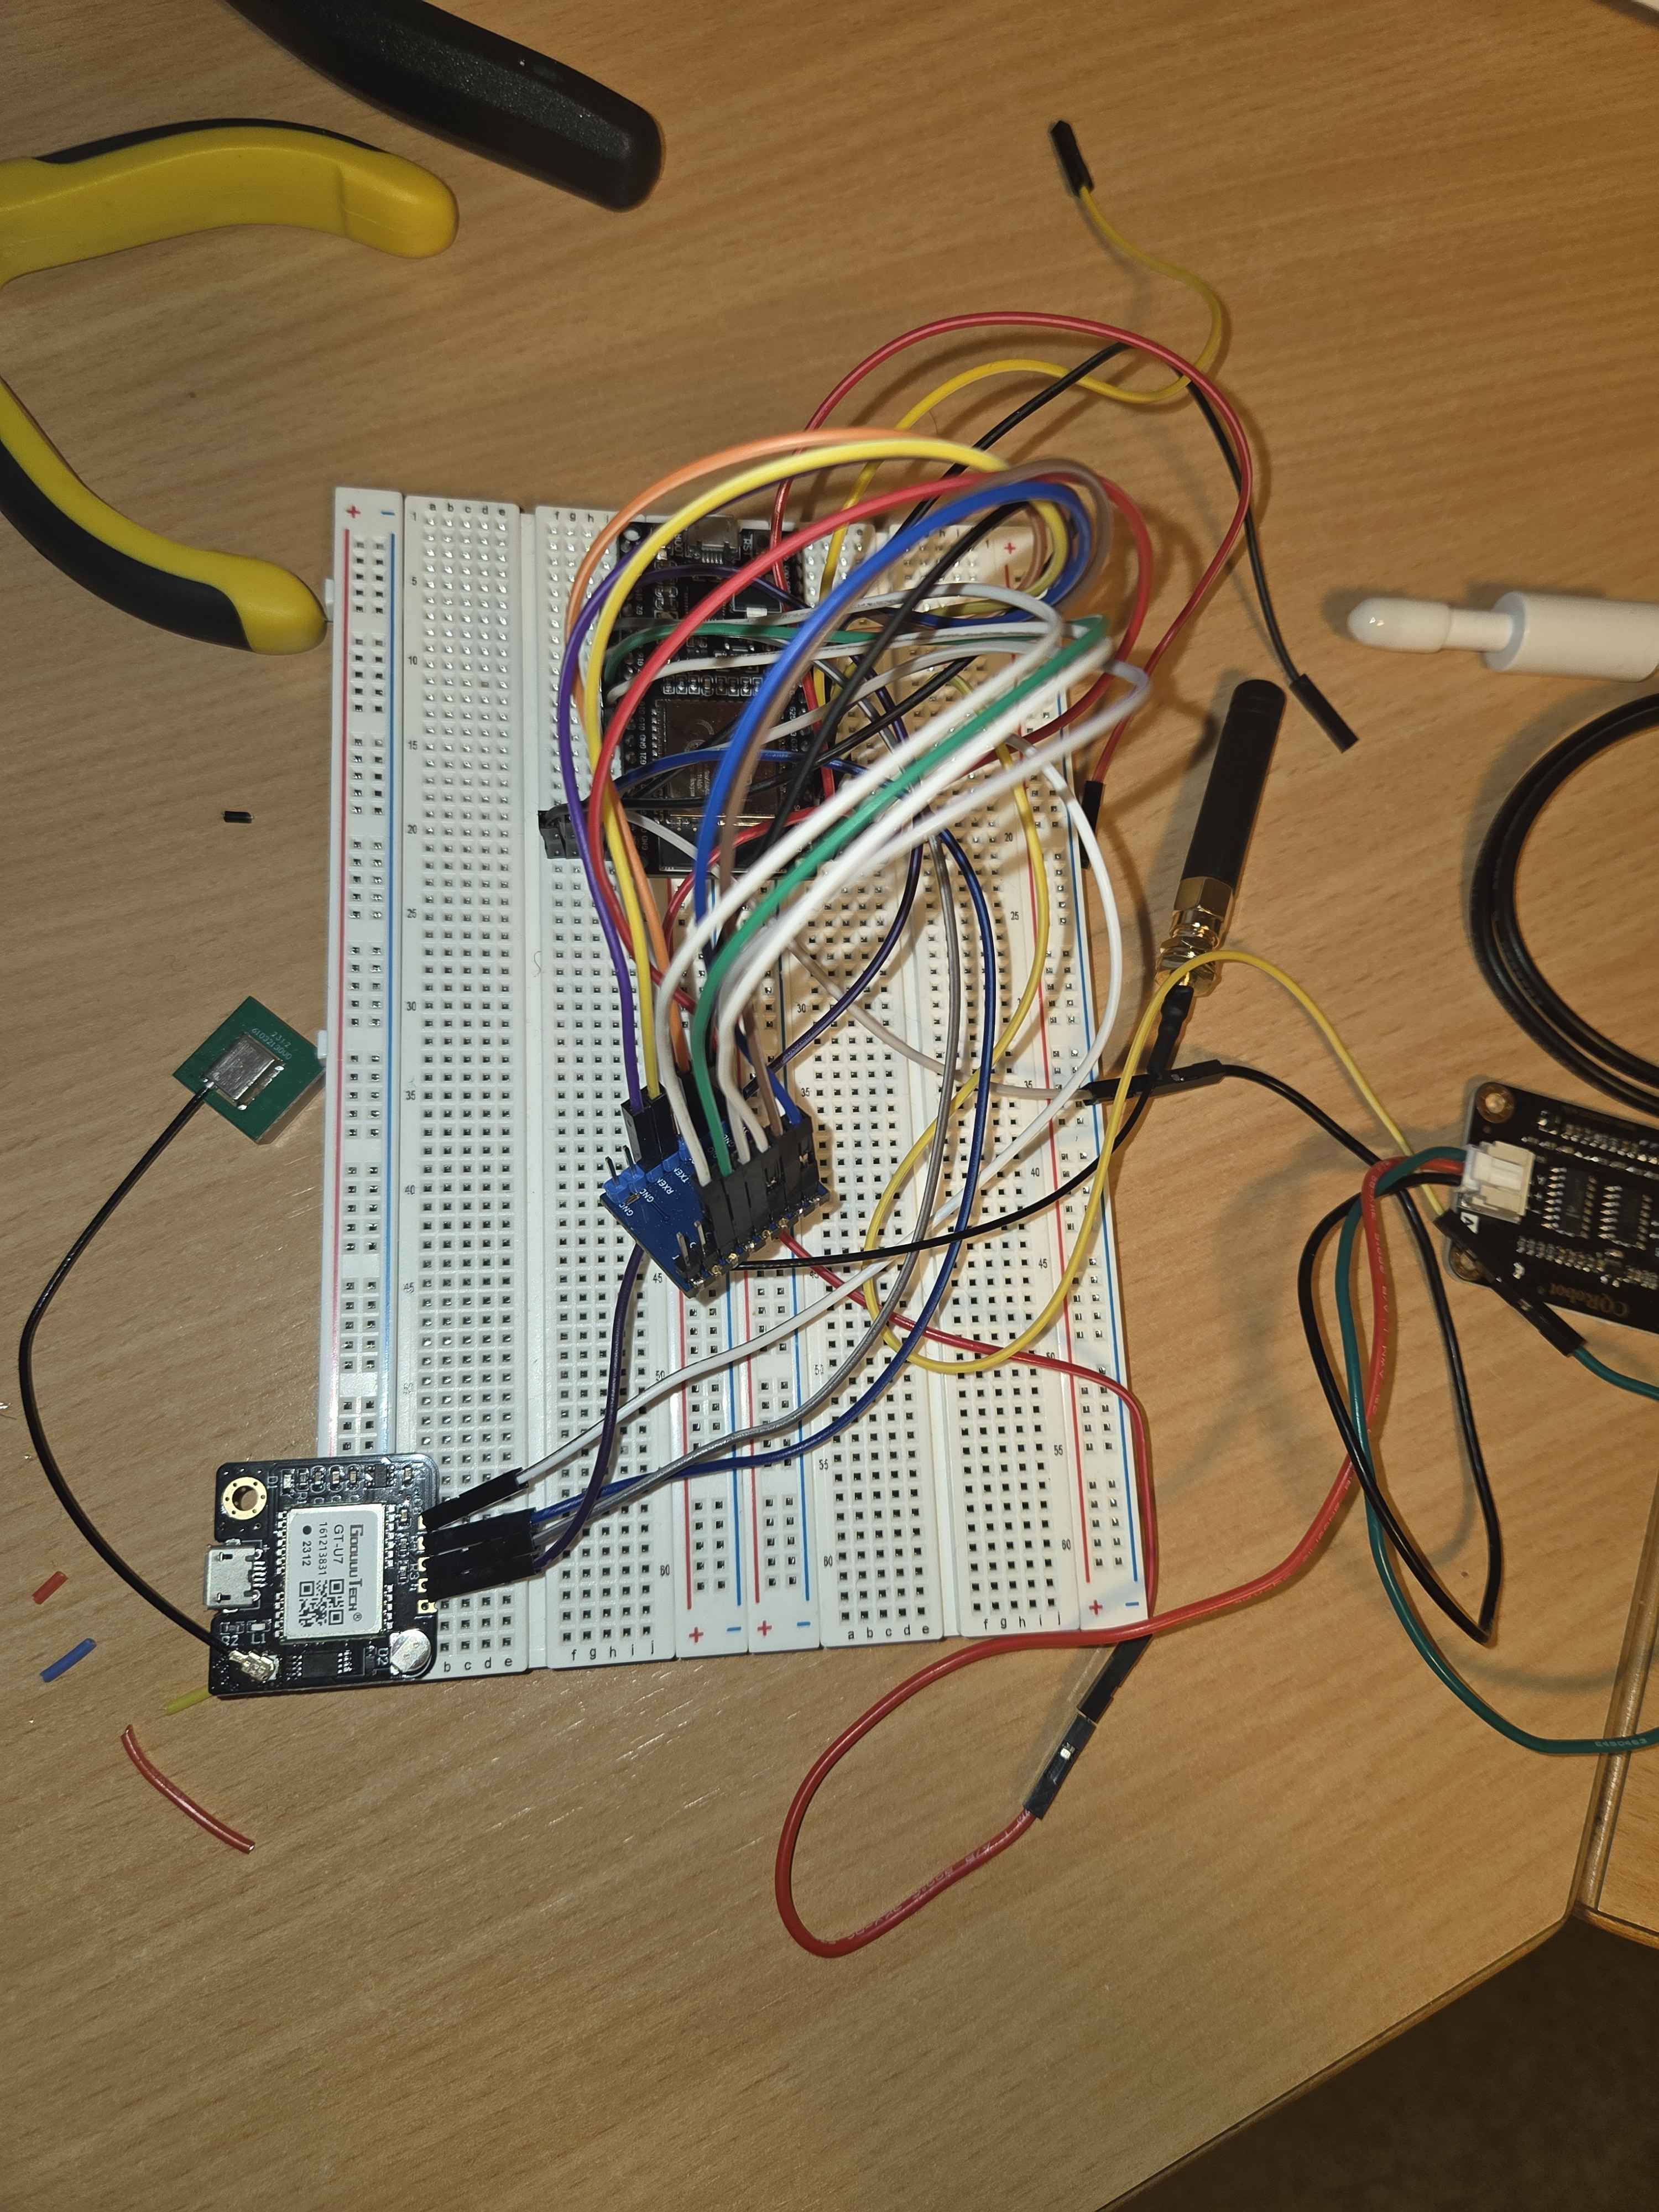
\includegraphics[width=\paperwidth,height=\paperheight,keepaspectratio]{material/I}}
\end{frame}
\begin{frame}[plain]
    \makebox[\linewidth]{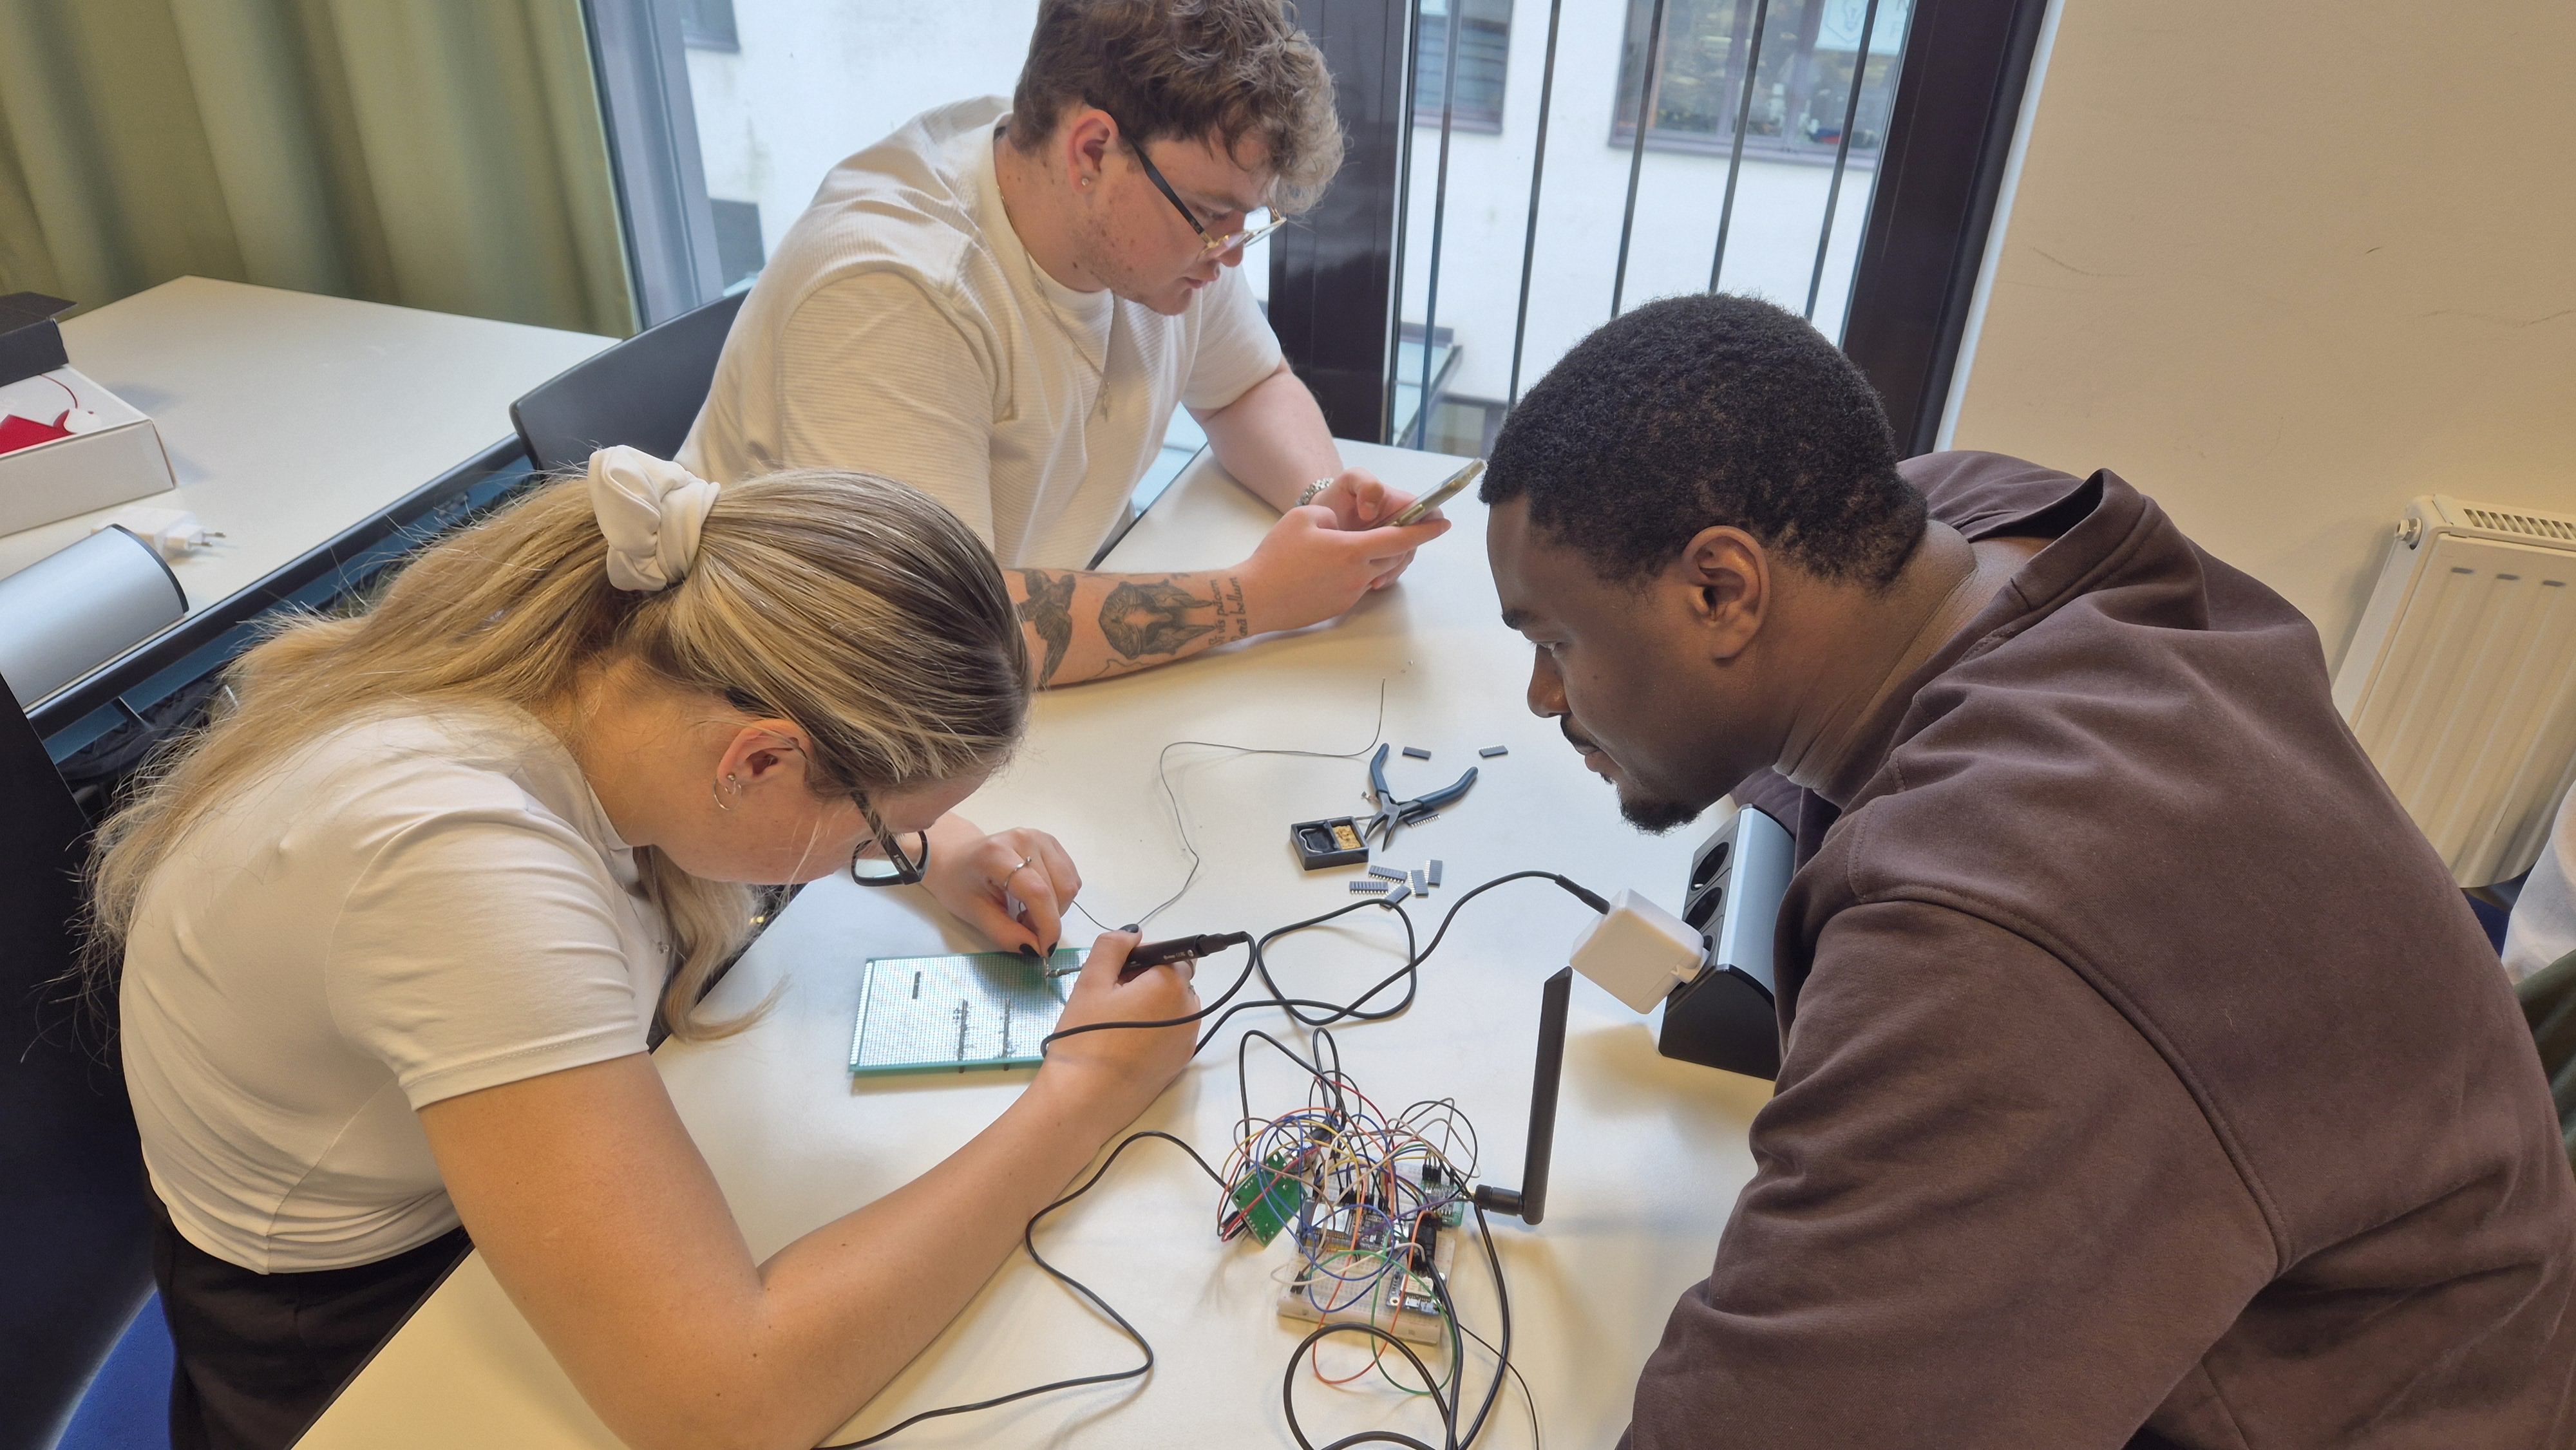
\includegraphics[width=\paperwidth,height=\paperheight,keepaspectratio]{material/I1}}
\end{frame}
\begin{frame}[plain]
    \makebox[\linewidth]{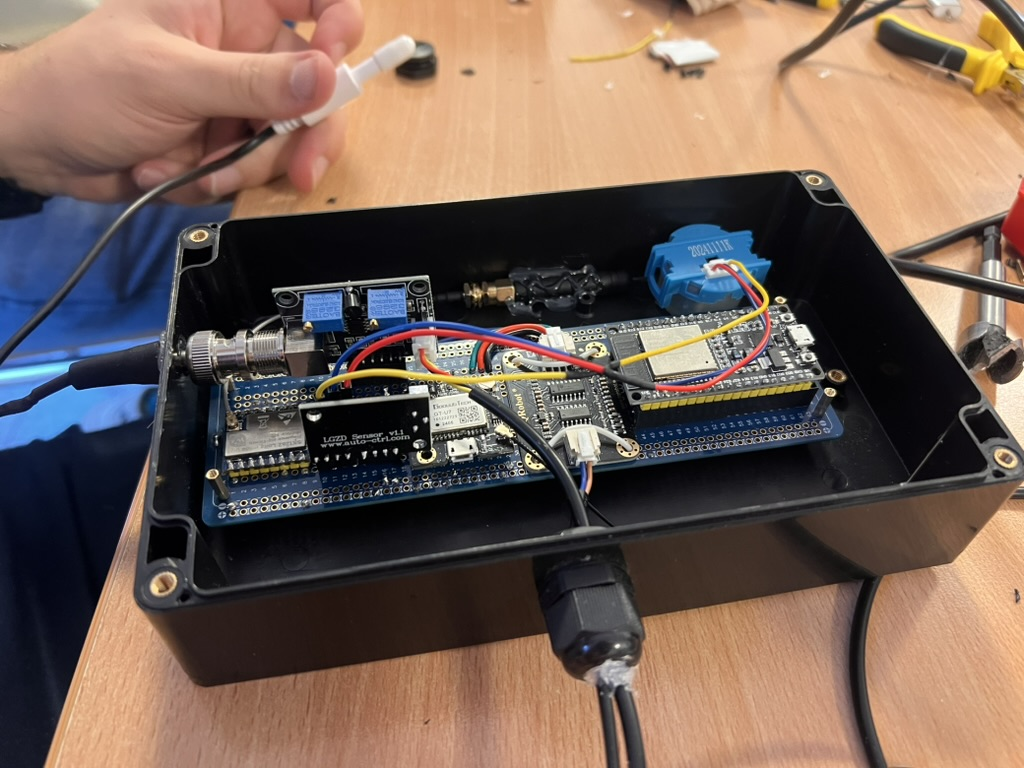
\includegraphics[width=\paperwidth,height=\paperheight,keepaspectratio]{material/J}}
\end{frame}
\begin{frame}[plain]
    \makebox[\linewidth]{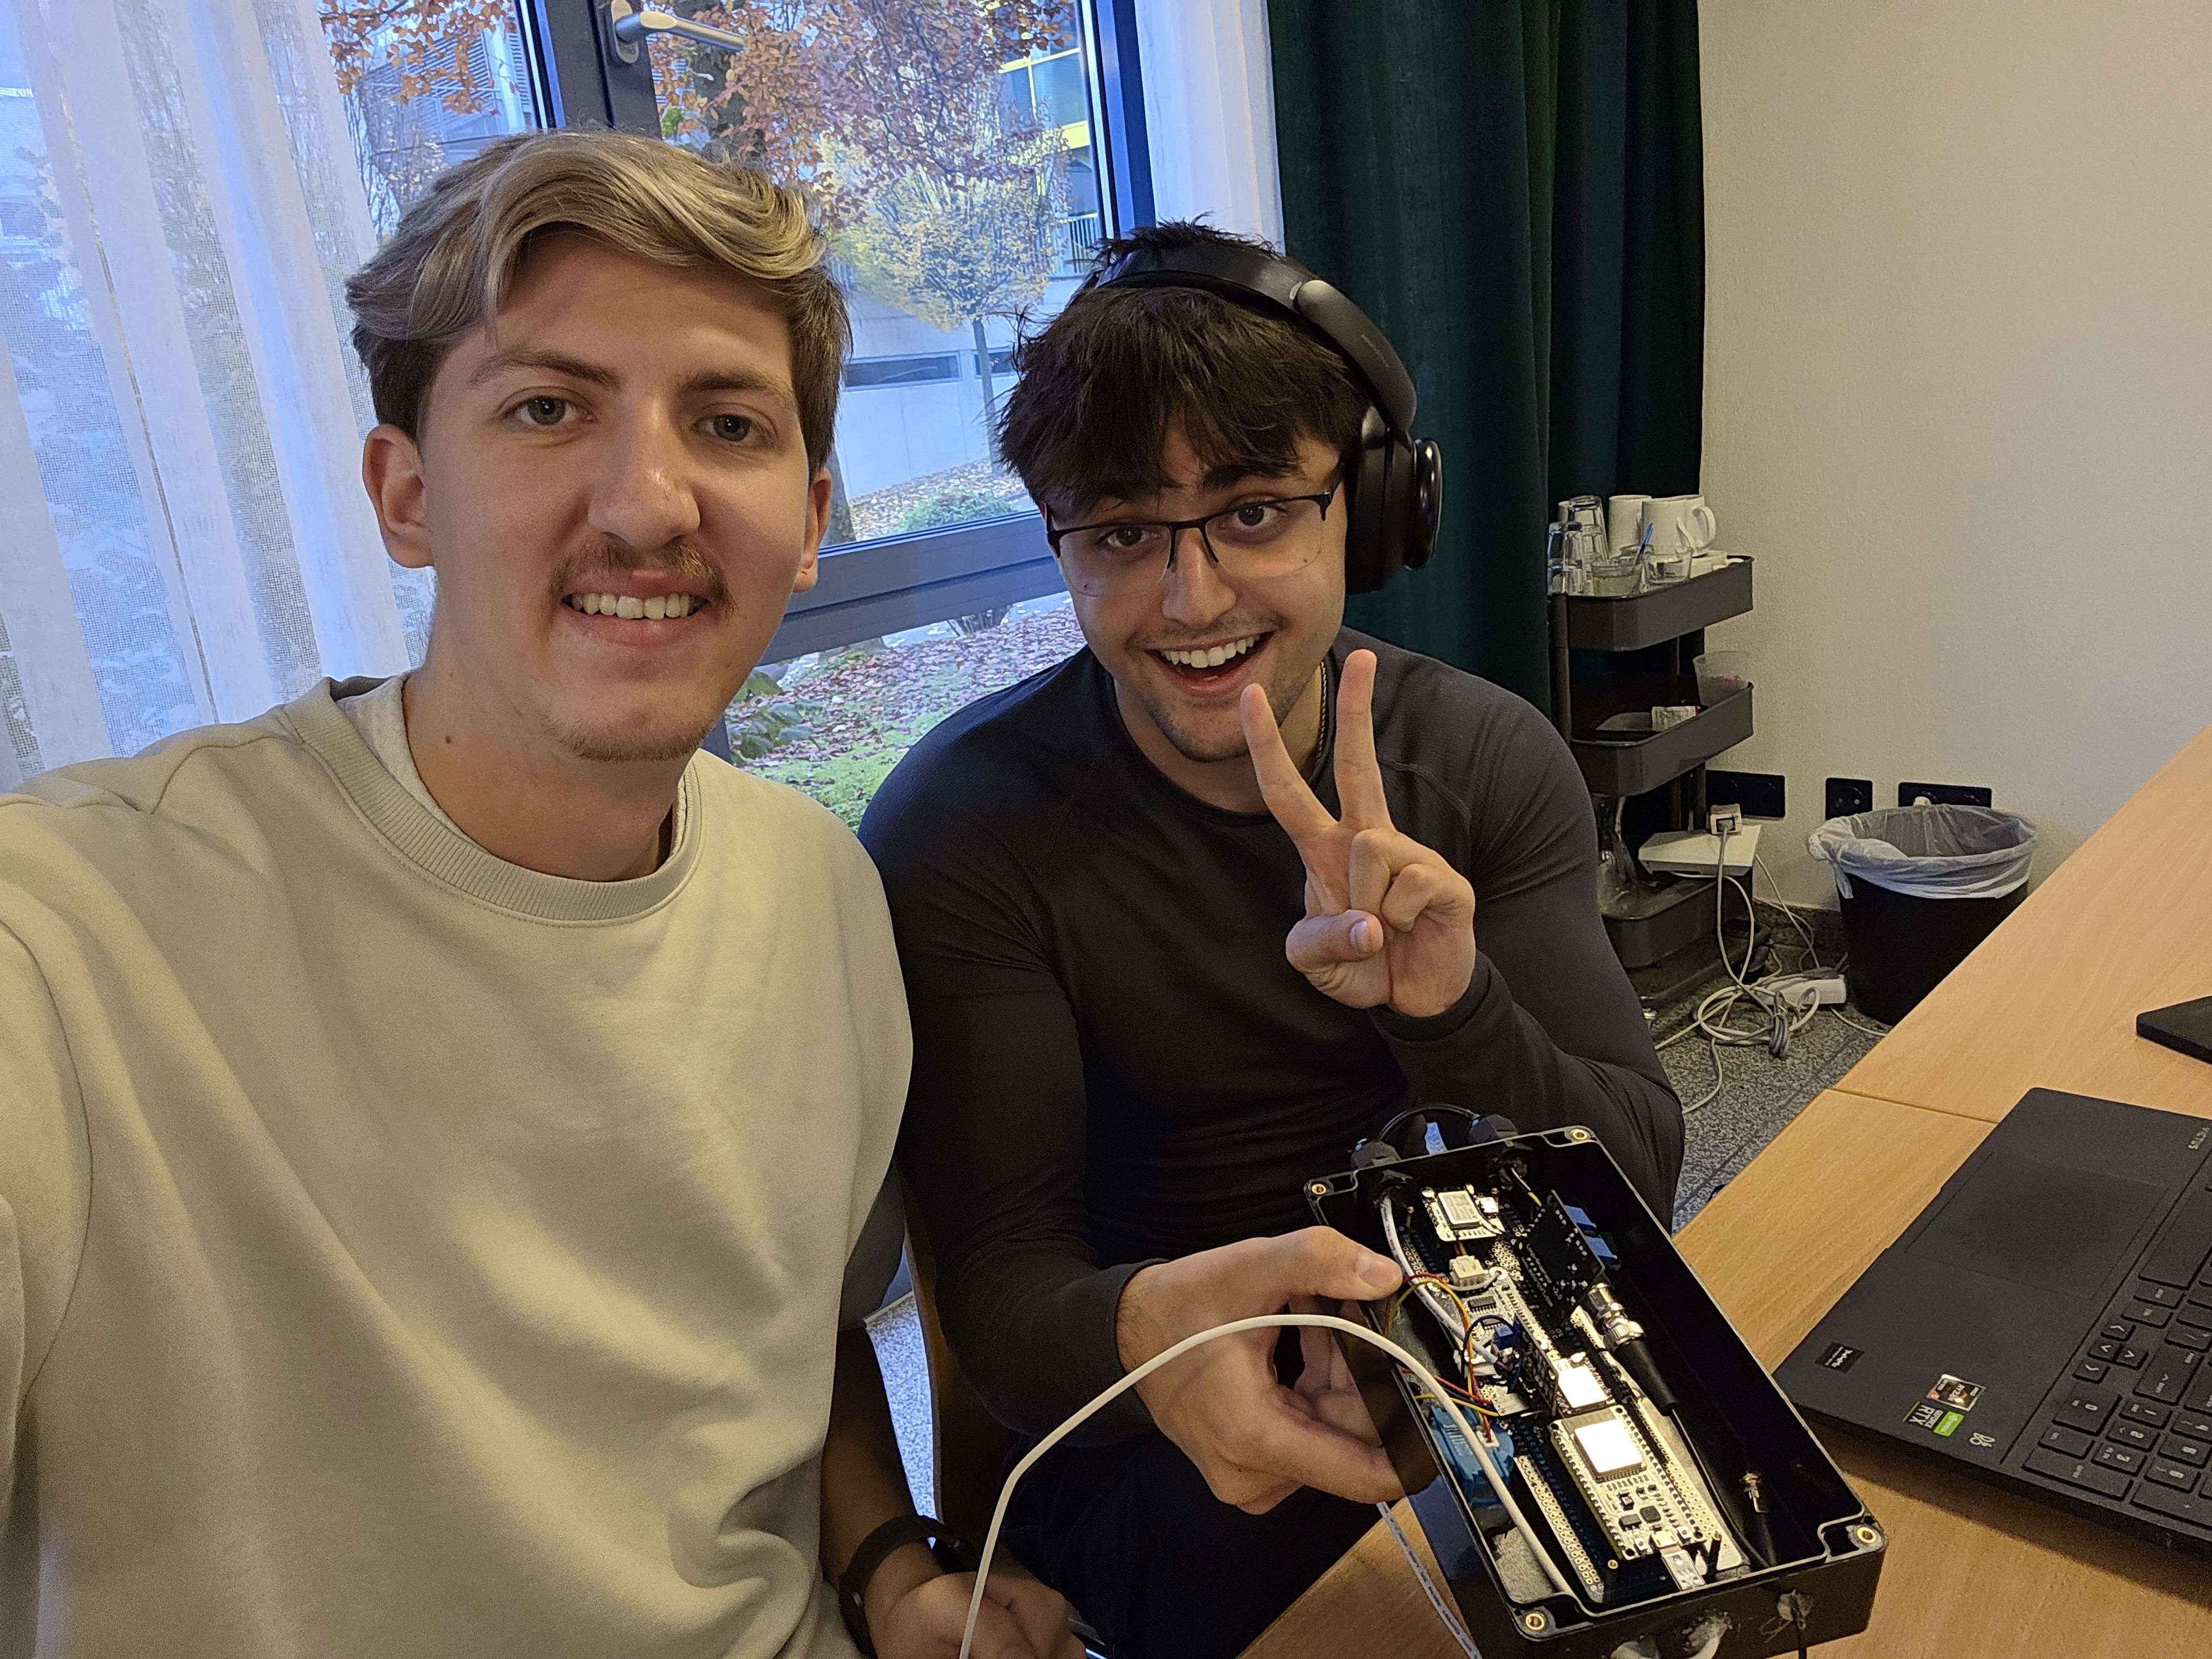
\includegraphics[width=\paperwidth,height=\paperheight,keepaspectratio]{material/K}}
\end{frame}
\setbeamercolor{normal text}{bg=white}
